\chapter{Special Topics}\label{ch:special}

\begin{quote}\ttfamily
	When you have a hammer in your hand, it's hard refraining yourself from treating everything as a nail.
\end{quote}
The objective of this chapter is to provide with some very powerful tools and some special topics, which are incredibly helpful. Some topics may not be very useful for solving problems, but they are quite good for making someone think and thus they encourage us to study more on them. Let's start with a really nice lemma.

\section{Thue's Lemma}
\documentclass{subfile}

\begin{document}
\textit{Thue's Lemma} is a wonderful theorem in modular arithmetic. It should have been quite popular, but unfortunately, it is not as well-known as it should be. Here we will see what a powerful tool it is.

\begin{theorem}[Thue's Lemma]\label{thm:thue}\slshape
	Let $n>1$ be an integer and $a$ be an integer coprime to $n$. Then, there are integers $x$ and $y$ so that 
	\begin{align*}
		0 &< |x|, |y| \leq \sqrt n, \quad \text{and}\\
		x&\equiv ay\pmod n.
	\end{align*}
	We call such a solution $(x,y)$ to the above congruence equation a \textit{small solution}.
\end{theorem}

\begin{proof}
	Let $r=\lfloor\sqrt{n}\rfloor$. That means $r$ is the unique integer for which $r^2\leq n<(r+1)^2$. The number of pairs $(x,y)$ of integers for which $0\leq x,y\leq r$, is $(r+1)^2$. This number is greater than $n$. Therefore, by pigeonhole principle, there must be two different pairs $(x_1,y_1)$ and $(x_2,y_2)$ among these $(r+1)^2$ pairs so that 
	\begin{align*}
		& x_1-ay_1 \equiv \ \ x_2-ay_2 \pmod n\\
		\implies & x_1-x_2 \ \equiv a(y_1-y_2) \pmod n.
	\end{align*}
	Let $x=x_1-x_2$ and $y=y_1-y_2$, so we get $x\equiv ay\pmod n$. We only need to show that $x$ and $y$ are non-zero (it is obvious that $|x|$ and $|y|$ are both less than or equal to $\sqrt n$). Certainly, if one of $x$ or $y$ is zero, the other is zero as well. If both $x$ and $y$ are zero, that would mean that two pairs $(x_1,y_1)$ and $(x_2,y_2)$ are actually the same. That is not the case because we first assumed that they are different pairs of integers. Therefore, neither $x$ nor $y$ is zero and we are done.
\end{proof}
	
	\begin{note}
		The condition $0<x,y<\sqrt{n}$ is important. Because of this condition, we can rule out trivial cases and bound the small solutions as the problems require.
	\end{note}
	
	\begin{corollary}\slshape
		For a prime $p$ and an integer $a$ coprime to $p$, there exist integers $x$ and $y$ with $0<|x|,|y|<\sqrt{p}$ such that
		\begin{align*}
			a & \equiv xy\pmod p.
		\end{align*}
	\end{corollary}
	
	This lemma can be generalized even more with the same proof.
	\begin{theorem}[Generalization of Thue's Lemma]\slshape
		Let $p$ be a prime number and let $\alpha$ and $\beta$ be two real numbers so that $\alpha\beta \geq p$. Then, for an integer $x$ relatively prime to $p$, there are integers $a$ and $b$ with $0<|a|<\alpha$ and $0<|b|<\beta $ so that
		\begin{align*}
			a & \equiv xb\pmod p.
		\end{align*} 
	\end{theorem}
	We can also generalize the latter theorem to a two-dimensional theorem.
	\begin{theorem}[Two-dimensional Thue's Lemma]\slshape
		Let $n\geq2$ be an integer and define $r=\sqrt{n}$. For arbitrary integers $a,b,c$, and $d$, there exist integers $w,x,y$, and $z$ with at least one of $y$ or $z$ non-zero such that
		\begin{align*}
			0& \leq |w|,|x|,|y|,|z|\leq r,\\
			w&\equiv ay+bz\pmod n, \quad \text{and}\\
			x&\equiv cy+dz\pmod n.
		\end{align*}
	\end{theorem}
	
	
	Now we demonstrate some applications of the lemma. First, we show an elegant proof of Fermat's $4n+1$ theorem, restated in theorem \autoref{thm:fermat4n+1}.
	
	\begin{theorem}[Fermat's Theorem on Sum of Two Squares]\label{thm:fermat4n+1}\slshape
		Any prime of the form $4n+1$ can be represented as a sum of two squares.
	\end{theorem}

	\begin{proof}
		We already know from theorem \autoref{thm:-1qr} that for $p\equiv1\pmod4$, there is an $x$ so that
		\begin{align*}
			x^2 & \equiv-1\pmod p.
		\end{align*}
		From Thue's lemma, for such an $x$, there are integers $a$ and $b$ with $0<|a|,|b|<\sqrt{p}$ so that
		\begin{align*}
			a \equiv xb \pmod p & \implies	a^2 \equiv x^2b^2 \equiv -b^2\pmod p\\
			& \implies	a^2+b^2 \equiv 0 \pmod p.
		\end{align*}
		The last congruence means that $p|a^2+b^2$, so
		\begin{align*}
			p   &\leq a^2+b^2\text {, but}\\
			a^2+b^2	&< p+p = 2p.
		\end{align*}
		Therefore, $a^2+b^2=p$ must occur.
	\end{proof}

	\begin{remark}
		We can prove a stronger result than that of Theorem \autoref{thm:fermat4n+1} using Fibonacci-Brahmagupta Identity (see Identity \ref{id:fibbr} in Appendix \ref{ch:appendices}). This identity states that
		\begin{align*}
			(a^2+nb^2)(c^2+nd^2)&=(ac-nbd)^2+n(ad+bc)^2\\
			&=(ac+nbd)^2+n(ad-bc)^2.
		\end{align*}
	Since we know that the product of any two numbers of the form $4k+1$ is again of the form $4k+1$ (see the proof of Theorem \ref{thm:4k+3prime}), the special case when $n=1$ of the above identity along with Theorem \ref{thm:fermat4n+1} shows that all numbers which are comprised only of prime divisors of the form $4k+1$ are representable as the sum of two squares. 
	\end{remark}
	In fact, we can use the same technique for generalizing theorem \autoref{thm:fermat4n+1}.
	\begin{theorem}\label{thm:gen4n+1}\slshape
		Let $n\in\{-1,-2,-3\}$. If $n$ is a quadratic residue modulo a prime $p$, then there are integers $a$ and $b$ so that $a^2-nb^2=p$.
	\end{theorem}
	
	\begin{proof}
		We have already proven the case $n=-1$. If $n$ is a quadratic residue modulo $p$, 
		\begin{align*}
			x^2\equiv n\pmod p
		\end{align*}
		has a solution. Fix the integer $x$ and take $a$ and $b$ as in Thue's lemma so that
		\begin{align*}
			a \equiv xb\pmod p &\implies a^2 \equiv x^2b^2 \equiv nb^2\pmod p\\
			& \implies p  |a^2-nb^2.
		\end{align*}
		
		\begin{enumerate}
			\item If $n=-2$, then $p\leq a^2+2b^2<p+2p=3p$. This means either $a^2+2b^2=p$ or $a^2+2b^2=2p$ occurs. If the first equation holds, we are done. If $a^2+2b^2=2p$, we see that $a$ must be even. Replace $a=2a'$ in the latter equation to get $p=b^2+2a'^2$, as desired.
			\item If $n=-3$, we find $p\leq a^2+3b^2<p+3p=4p$. If $a^2+3b^2=2p$, then $a$ and $b$ are both odd or both even. If both are even, then $2p$ is divisible by $4$, a contradiction since $p$ is odd. Otherwise, $a$ and $b$ are both odd:
			\begin{align*}
				a^2+3b^2 & \equiv1+3\cdot 1\pmod 4\\
				\implies 2p	 & \equiv 0 \pmod 4.
			\end{align*}
			This is, again, a contradiction. We are left with the case $a^2+3b^2=3p$. This shows $a$ is divisible by $3$. If we take $a=3a'$, we easily observe that $p=b^2+3a'^2$.
		\end{enumerate}
	\end{proof}

	\begin{question}
		Can you prove a similar result to that of the remark after Theorem \autoref{thm:fermat4n+1}, but for the above theorem? Try using Fibonacci-Brahmagupta's identity before reading the next corollary.
	\end{question}
	
	\begin{corollary}\label{cor:p|x^2+ny^2}\slshape
		For a prime $p$ and an integer $n$ with $p \nmid n$ the following two statements are equivalent:
		\begin{itemize}
			\item There exist coprime integers $x$ and $y$ so that $p$ divides $x^2+ny^2$.
			\item $-n$ is a quadratic residue modulo $p$.
		\end{itemize}
	\end{corollary}
	
	\begin{proof}
		First, assume that $p|x^2+ny^2$. Then, $y$ must be coprime to $p$. Therefore, $y$ has an inverse modulo $p$, say $a$. So, $ay\equiv1\pmod p$. Then, $a^2y^2  \equiv1\pmod p$, and
		\begin{align*}
			p | x^2 + ny^2 &\implies p |a^2x^2+na^2y^2\\
			& \implies p |a^2x^2+n\\
			& \implies (ax)^2 \equiv-n\pmod p.
		\end{align*}
		Now, suppose that $-n$ is a quadratic residue modulo $p$. Let $k^2\equiv-n\pmod p$. Clearly, $(k,p)=1$, otherwise $p$ will divide $n$. From Thue's lemma, there are integers $x$ and $y$ such that 
		\begin{align*}
			x \equiv ky\pmod p & \implies x^2 \equiv k^2y^2 \equiv-ny^2\pmod p\\
			&\implies  p |x^2+ny^2.
		\end{align*}
	\end{proof}
	We can use these results to imply the following theorem.
	\begin{theorem}
		For $D\in\{1,2,3\}$, if $n=x^2+Dy^2$ for some coprime integers $x$ and $y$, then every divisor $d$ of $n$ is of the same form as $n$.
	\end{theorem}
	
	\begin{proof}
		According to the Fibonacci-Brahmagupta Identity (identity \autoref{id:fibbr} in appendix \autoref{ch:null}),
			\begin{align*}
				(a^2+Db^2)(c^2+Dd^2)& =(ac-Dbd)^2+D(ad+bc)^2\\
				& =(ac+Dbd)^2+D(ad-bc)^2.
			\end{align*}
		This means that the product of two numbers of the form $x^2+Dy^2$ is of the same form. From theorems above, if $p$ is a divisor of $x^2+Dy^2$, then $p=a^2+Db^2$ for some integers $a$ and $b$. The identity clearly says that if $m=a^2+Db^2$, then any power of $m$, say, $m^k$, is of this form again. Let's assume that the prime factorization of $n$ is
			\begin{align*}
				n & = p_1^{e_1}\cdots p_k^{e_k} = \prod_{i=1}^{k}p_i^{e_i}.
			\end{align*}
		Then, since $d$ is a factor of $n$, the factorization of $d$ is
			\begin{align*}
				d & = \prod_{i=1}^{k}p_i^{f_i}\text{ where }0\leq f_i\leq e_i.
			\end{align*}
		For any $1\leq i\leq k$, $p_i$ divides $n=x^2+Dy^2$. Therefore, according to corollary \autoref{cor:p|x^2+ny^2}, $-D$ is a quadratic residue modulo $p_i$. Now, by theorem \autoref{thm:gen4n+1}, each $p_i$ is of the form $x^2+Dy^2$. From our previous discussion, we find that $p_i^{f_i}$ is of the same form for all $i$. As a consequence, the product $p_1^{f_1}\cdots p_k^{f_k}=d$ is of the same form and we are done.
	\end{proof}
	Now we prove another theorem that demonstrates the power of Thue's lemma. We will use a theorem which we proved in section \autoref{sec:qr}. For convenience, we state the theorem here again.
		\begin{theorem}\slshape
			$-3$ is a quadratic residue modulo $p$ if and only if $p$ is of the form $3k+1$.
		\end{theorem}
	Using this theorem, we will prove the following.
		\begin{theorem}\slshape
			If $p$ is a prime of the form $3k+1$, there are integers $a$ and $b$ such that $p=a^2+ab+b^2$.
		\end{theorem}
	
	\begin{proof}
		Since $p$ is of the form $3k+1$, $-3$ is a quadratic residue of $p$. Take $y$ to be an odd integer for which $p|y^2+3$ or,
			\begin{align*}
				y^2 & \equiv-3\pmod p.
			\end{align*}
		Such an $y$ exists since $p$ is odd. Then, the congruence equation $y\equiv2x+1\pmod p$ has an integer solution for $x$. For that $x$, we get
			\begin{align*}
				(2x+1)^2 & \equiv-3\pmod p\\
				4x^2+4x+1& \equiv-3\pmod p\\
				4(x^2+x+1)&\equiv 0 \phantom{-}\pmod p\\
				x^2+x+1	 & \equiv 0 \phantom{-}\pmod p.
			\end{align*}
		The latter congruence equation holds because $p$ is odd. From Thue's lemma, there are integers $a$ and $b$ with $0<|a|,|b|< \sqrt p$ such that
			\begin{align*}
				a & \equiv xb\pmod p.
			\end{align*}
		Then,
			\begin{align*}
				a^2+ab+b^2  & \equiv (xb)^2+(xb)\cdot b+b^2\\
				& \equiv b^2(x^2+x+1)\\
				& \equiv 0\pmod p.
			\end{align*}
		Since $p|a^2+ab+b^2$, we have $p\leq a^2+ab+b^2$. On the other hand,
			\begin{align*}
				p& \leq a^2+ab+b^2 \\
				& < p+p+p \\
				&= 3p.
			\end{align*}
		Consequently, either $a^2+ab+b^2=p$ or $a^2+ab+b^2=2p$ happens. We can easily check that $a^2+ab+b^2=2p$ can not happen (try it yourself). Thus, $a^2+ab+b^2=p$, which is what we wanted.
	\end{proof}
	
	You have probably figured out by now that \textbf{our focus should be on the small solutions} so that we can bound the necessary expressions like the problem asks for. Let's see more examples on this.
	
	\begin{theorem}\slshape
		Let $p>5$ be a prime which divides $k^2+5$ for some integer $k$. Show that there are integers $x$ and $y$ such that $p^2=x^2+5y^2$.
	\end{theorem}
	
	\begin{hint}
		Try to find $x$ such that $x^2\equiv-5\pmod{p^2}$. Then from Thue's lemma, there exist $a$ and $b$ so that $a^2,b^2<p$ and $a\equiv kb\pmod{p^2}$. This gives $a^2\equiv k^2b^2\equiv-5b^2\pmod{p^2}$. Now, check all the cases like we did before.
	\end{hint}
	
	\begin{problem}
		Let $p$ be a prime for which there exists a positive integer $a$ such that $p$ divides $2a^2-1$. Prove that there exist integers $b$ and $c$ so that $p=2b^2-c^2$.
	\end{problem}
	
	\begin{solution}
		Let's look for small solutions again for the purpose of bounding! We have $2a^2-1\equiv0\pmod p$. Since we want to bound $2b^2-c^2$, it is obvious that we must find $b$ and $c$ so that $p$ divides $2b^2-c^2$ and then bound it. Fix the integer $a$, which is clearly coprime to $p$. Then from Thue's lemma, we there are integers $b$ and $c$ with $0<|b|,|c|<\sqrt{p}$ so that
		\begin{align*}
			b & \equiv ac\pmod p.
		\end{align*}
		This gives us what we need. Note that
		\begin{align*}
			2b^2-c^2 & \equiv 2(ac)^2-c^2\\
			& \equiv c^2(2a^2-1)\\
			& \equiv 0\pmod p.
		\end{align*}
		Thus, $p$ divides $2b^2-c^2$, and now we get to use the fact that
		\begin{align*}
			p & \leq 2b^2-c^2\\ 
			& < 2b^2 \\
			& < 2p.
		\end{align*}
		We immediately get that $p=2b^2-c^2$.
	\end{solution}

	
\end{document}

\section{Chicken McNugget Theorem}
\documentclass{subfile}

\begin{document}
	You are probably wondering how come this can be the name of a theorem if you have encountered it for the first time. The name just might be the weirdest of all names a theorem can possibly assume! Here is the reason behind such a name: The story goes that the Chicken McNugget Theorem got its name because in McDonalds, people bought Chicken McNuggets in 9 and 20 piece packages. Somebody wondered what the largest amount you could never buy was, assuming that you did not eat or take away any McNuggets. They found the answer to be 151 McNuggets, thus creating the Chicken McNugget Theorem. Actually it is \textit{Sylvester's Theorem}, now known as the \textit{Chicken McNugget Theorem}. The problem is known as \textit{Frobenius Coin Problem}, which is a generalization of this one. Have you ever wondered about the coin system of your own country? It is designed in a way so that you should never face a situation where you can not exchange a certain amount of money. But have you thought how it is possible? In this section, we will deal with problems like this. First think for yourself on the following two problems:
		\begin{problem}
			You are in a strange country where only two units are available for exchange: $4$ and $6$. Can you pay any amount you want?
		\end{problem}

		\begin{problem}
			In another country, you see that only two units are available for exchange: $3$ and $10$. Can you pay any amount you want?
		\end{problem}

	If you have come to the right conclusions, you will see that you can not pay any amount you want in the first case. But you can pay whatever you want with the second one. Let's say two units available value $a$ and $b$. So if you use $a$ unit $x$ times and $b$ unit $y$ times, the total amount of money you can pay is $ax+by$. Here, $x,y$ can be negative or non-negative integers. If $x>0$, it will mean you are paying, or if $x<0$ it will mean you are being paid (or getting the exchange). Therefore, if you need to pay exactly $n$ amount, you need integers $x$ and $y$ with
		\begin{align*}
			ax+by & = n
		\end{align*}
	Play with some more values of $a$ and $b$. You will understand that you can pay $n$ amount with units $a$ and $b$ if and only $(a,b)$ divides $n$. Here is another intuitive fact: If we can pay just $1$, we can pay any amount we want with as many $1$s needed. So we should focus on when we can pay $1$ by $a$ and $b$. This tells us, $a$ and $b$ must be co-prime. And from B\'{e}zout's Identity, for any co-prime $a$ and $b$, we will get integers $x,y$ so that
		\begin{align*}
			ax+by & = 1
		\end{align*}
	In the problems above, we can't pay any amount with $4$ and $6$ because they are not co-prime. But we can pay any amount that is a multiple of $(4,6)=2$. But we can pay any amount with $3$ and $10$ because they are co-prime. This leads us to the following theorem.

	\begin{theorem}
		Any integer can be written as a linear combination of $a$ and $b$ if and only if $a\perp b$.
	\end{theorem}
By linear combination, we mean using only $a$ and $b$ as many times as we want. Now we see the same problem from another perspective. Consider the following problem. If $n$ can be written as $ax+by$ for non-negative $x,y$, we will call $n$ a \textit{good} number. Otherwise, $n$ is \textit{bad}. But to do that, we can't change the values of $a$ and $b$ simultaneously. Therefore, we fix two co-prime integers $a$ and $b$. Next, let's see why we are only considering $a\perp b$. If $(a,b)=g$ and $g>1$, then we already know that only multiples of $g$ can be good. But we want as many integers to be good as possible, and not skipping some integers is better.
	\begin{problem}
		A shop sells nuggets in packages of two sizes, $3$ nuggets and $10$ nuggets. What is the maximum number of nuggets that cannot be expressed as a nonnegative combination of these package sizes?
	\end{problem}

	\begin{definition}[Frobenius Number]
		For two integers $a$ and $b$, the largest bad integer is the \textit{Frobenius number}. In fact, it can be generalized for $n$ natural numbers. If $a_1,\ldots,a_n$ are natural numbers so that $(a_1,\ldots,a_n)=1$, the largest natural number that can not be written as $a_1x_1+\ldots a_nx_n$ for nonnegative $x_1,\ldots,x_n$ is the Frobenius number. It is denoted as $F_n(a_1,\ldots,a_n)$. Here, we will deal with the case $n=2$, $F_2(a,b)$.
	\end{definition}
The following theorem answers this question.
	\begin{theorem}[Sylvester's Theorem, 1882]
		Let $a$ and $b$ be two co-prime positive integers greater than $1$. Then the maximum integer that can not be expressed as $ax+by$ for non-negative integer $x,y$ is $ab-a-b$.
	\end{theorem}
If we can prove that for all $N>ab-a-b$, there are non-negative integers $x,y$ such that
	\begin{align*}
		N & = ax+by
	\end{align*}
and that for $N\leq ab-a-b$, there are no such $x$ and $y$, we are done. First, let's prove the next lemma.
	\begin{lemma}
		$ab-a-b$ is a bad number.
	\end{lemma}

	\begin{proof}
		On the contrary, let's assume that
			\begin{align*}
				ab-a-b & = ax+by
			\end{align*}
		for some $x,y\in\mathbb{N}_0$. We can rewrite it as
			\begin{align*}
				a(x-b+1) & = -b(y+1)
			\end{align*}
		From this equation, $a\mid b(y+1)$ but $a\perp b$. So, $a|y+1$. Again, $b\mid a(x-b+1)$ but $b\perp a$ so $b\mid x-b+1$ or $b\mid x+1$. We get $x+1\geq b$ and $y+1\geq a$, and so
			\begin{align*}
				 x
				 	& \geq b-1\\
				 y
				 	& \geq a-1
			\end{align*}
		Using these inequalities,
			\begin{align*}
				 ax+by
				 	& \geq a(b-1)+b(a-1) \\
					&= ab-a+ab-b\\
				\implies ab-a-b
					& \geq 2ab-a-b
			\end{align*}
		which is a contradiction.
	\end{proof}

%	\begin{lemma}
%		If $m$ and $n$ both are good, then so is $m+n$.
%	\end{lemma}
%
%	\begin{proof}
%		If $m$ and $n$ are good, then there are nonnegative integers $x,y,u$ and $v$ so that
%			\begin{align*}
%				m & = ax+by, \text{ and }\\
%				n & = au+bv.
%			\end{align*}
%		Therefore, $m+n= a(x+u)+b(y+v)$ is good.
%	\end{proof}
%
%	\begin{lemma}
%		If $m+n=ab-a-b$, then exactly one of $m$ and $n$ is good.
%	\end{lemma}
%
%	\begin{proof}
%		If both $m$ and $n$ are good, then according to the lemma above, $m+n$ is good too. But that would contradict the fact that $ab-a-b$ is bad. So, one of $m$ or $n$ must be bad.
%	\end{proof}
The above lemma shows that $F_2(a,b) \geq ab-a-b$. It only remains to prove the following lemma:
	\begin{lemma}
		Any integer $n>ab-a-b$ is good.
	\end{lemma}

	\begin{proof}
		Since $(a,b)=1$, by B\'{e}zout's identity, there are integers $u$ and $v$ so that
			\begin{align}
				au+bv
					& = 1\\
				\implies anu+bnv
					& = n\nonumber\\
				\implies ax_0+by_0
					& = n\label{eqn:syl1}
			\end{align}
		We need to show that such $x_0,y_0 \geq 0$ exist. If $(x_0,y_0)$ is a solution of equation \eqref{eqn:syl1}, then so is $(x_0-bt,y_0+at)$ for any integer $t$. Here, one can choose $t$ such that $0 \leq x_0-bt<b$. In case you don't understand how we can choose such $t$, just divide $x_0$ by $b$. Then $x_0=bq+r$, where $0\leq r <b$. This means that $0 \leq x_0 -bq <b$, so one choice for $t$ is $q$. So we know that there exists some $x_0$ such that $0 \leq x_0<b$. We will show that $y_0$ is also positive. Note that
			\begin{align*}
				ax_0+by_0
					& = n\\
					& > ab-a-b\\
				\implies b(y_0+1)
					& > a(b-x_0-1)
			\end{align*}
		Since we know that $x_0<b$, we get $b-x_0-1\geq 0$. This means that $b(y_0+1) >0$, so $y_0+1>0$, i.e., $y\geq0$. Therefore, there is a valid solution $(x_0,y_0)$ and the proof is complete.
	\end{proof}
Now, the proof is complete. The same proof can be used for generalizing the case where $(a,b)>1$.
	\begin{theorem}[Generalization of Sylvester's Theorem]
		Let $a,b$ be positive integers with $(a,b)=g$. Then every integer
			\begin{align*}
				n\geq\dfrac{(a-g)(b-g)}{g}
			\end{align*}
		such that $g|n$ is good. Also,
			\begin{align*}
				F_2(a,b)=\dfrac{(a-g)(b-g)}{g}-g
			\end{align*}
		i.e., $F_2(a,b)$ is the largest non-trivial bad integer.
	\end{theorem}

We see some problems related to this theorem. A classical example would be the following problem that appeared at the IMO $1983$.
	\begin{problem}[IMO 1983]
		Let $a,b,c\in\mathbb{N}$ with $(a,b)=(b,c)=(c,a)=1$. Prove that, $2abc-ab-bc-ca$ is the largest integer that can not be expressed as $xbc+yca+zab$ for non-negative $x,y,z$.
	\end{problem}

	\begin{solution}
		Clearly, we need to invoke Sylvester's theorem here. But the expression tells us, it can not be done in one step. Note that
			\begin{align*}
				xbc+yca+zab & = c(bx+ay)+zab
			\end{align*}
		Therefore, we should first focus only on $bx+ay$ first. From McNugget theorem, any integer greater than $ab-a-b$ is good. So we substitute $ab-a-b+1+t$ for some non-negative $t$ into the equation and get
			\begin{align*}
				xbc+yca+zab & = c(bx+ay)+zab\\
							& = c(ab-a-b+1+t)+zab\\
							& = abc-bc-ca+c+ct+zab
			\end{align*}
		This again calls for using the theorem for $c$ and $ab$. Again, every integer greater than $abc-ab-c$ is good. So we substitute $ct+zab=abc-ab-c+1+w$ for some non-negative $w$. Then
			\begin{align*}
				xbc+yca+zab & = abc-bc-ca+c+ct+zab\\
							& = abc-bc-ca+c+abc-ab-c+1+w\\
							& = 2abc-ab-bc-ca+1+w
			\end{align*}
	\end{solution}
This shows that all integers greater than $2abc-ab-bc-ca$ are good.	Finally, in order to prove the claim, we just have to show that $2abc-ab-bc-ca$ is bad. To the contrary, assume that $2abc-ab-bc-ca=xbc+yca+zab$ for some non-negative $x,y,z$. We have
	\begin{align*}
		bc(x+1)+ca(y+1)+ab(z+1)=2abc
	\end{align*}
Clearly, $a\mid x+1$ because $a|bc(x+1)$ but $\gcd(a,bc)=1$. Similarly, $b\mid y+1$ and $c\mid z+1$. This gives us $bc(x+1)+ca(y+1)+ab(z+1)\geq bca+cab+abc$ or $2abc\geq3abc$ which is obviously wrong.

So, the problem is solved. As you can see, the theorem is fairly easy to understand and use in problems. There will be some related problems in the problem column. See if you can get how to solve those using this (first you have to understand that this theorem will come to the rescue though).


\end{document}

\section{Vietta Jumping}
\documentclass{subfile}



\begin{document}
	By now, \textit{Vietta jumping} has become a standard technique for solving some particular type of olympiad number theory problems. It is also known as \textit{Root Jumping} or \textit{Root Flipping}. Though it involves Diophantine equations and for now, it is out of our scope, many divisibility or congruence problems can be turned into one that can be solved using this tactic. Hence, this section.
	To understand just how popular it has been, let's just mention that there are at least two IMO problems that have standard solutions using this particular technique. And surely, there are many other olympiad problems that fall into the same category. Now, let's see what it is and what it actually does.
	
	Consider the following quadratic equation
		\begin{align*}
		 	ax^2+bx+c & = 0.
		\end{align*}
	According to Vietta's formula, if two of its roots are $x_1$ and $x_2$, then
		\begin{align*}
			x_1+x_2 & = -\dfrac{b}{a}, \text{ and }\\
			x_1x_2  & = \dfrac{c}{a}.
		\end{align*}
	Vietta jumping relies on these two equations. It is in fact, a \textit{descent} method in which we usually prefer using one of the following two methods:
		\begin{enumerate}[(i)]
			\item \textbf{Standard Descent:} It is usually used to show that the equation doesn't have any solution or some sort of contradiction to prove a claim, like we do in \textit{Infinite Descent}. For a solution $(x,y)$ of the equation, we define a function dependent on $x,y$ ($x+y$ is such a common function, as we will see later). Then we consider the solution that minimizes that function over all solutions possible. If there are multiple solutions that can achieve this, we are free to choose any one depending on the problem. But then, using Vietta's formulas, we try to find another solution that makes the function's value smaller, which gives us the necessary contradiction. So, this is a modified version of infinite descent.
			\item \textbf{Constant Descending:} Sometimes, we take some constants, for example, an integer $k$ and fix it for the whole problem. For a solution $(a,b)$, we fix $b$ and $k$. Then using those formulas, we find a solution $x$ so that $0<x<b$ so that it produces a solution $(b,x)$ smaller than $(a,b)$. Note that, here, we have to take $b<a$ so that the new solution is guaranteed to be smaller. Repeating this, we will reach a base case and those constants ($k$, for example) will remain constant through the whole process. Thus, we will show what's required.
			\item Sometimes, there can be even geometric interpretations. For example, \textit{Arthur Engel} showed one in his book \textit{Problem Solving Strategies} chapter $6$, problem $15$.
		\end{enumerate}
	We will now demonstrate this using some example problems. Let's start with the classical problem from IMO $1988$. Here is what Engel said about this problem in his book:
		\begin{quote}\slshape
			Nobody of the six members of the Australian problem committee could solve it. Two of the members were George Szekeres and his wife Esther Klein, both famous problem solvers and problem creators. Since it was a number theoretic problem it was sent to the four most renowned Australian number theorists. They were asked to work on it for six hours. None of them could solve it in this time. The problem committee submitted it to the jury of the XXIX IMO marked with a double asterisk, which meant a superhard problem, possibly too hard to pose. After a long discussion, the jury finally had the courage to choose it as the last problem of the competition. Eleven students gave perfect solutions.
		\end{quote}
	
	\begin{problem}[IMO 1988, Problem 6]
		Let $ a$ and $ b$ be two positive integers such that $ab + 1$ divides $ a^{2} + b^{2}$. Show that $\dfrac{a^{2}+b^{2}}{ab+1}$ is a perfect square.
	\end{problem}
	
	\begin{solution}
		Let $k$ be an integer so that
			\begin{align*}
				&\dfrac{a^2+b^2}{ab+1} = k \\
				 \implies & a^2+b^2 = kab+k\\
				\implies  & a^2-kab+b^2-k = 0.
			\end{align*}
		As we said in the process, we will fix $k$ and consider all pairs of integers $(a,b)$ that gives us $k$ as the quotient. And take a solution $(a,b)$ in nonnegative integers so that the sum $a+b$ is minimum (and if there are multiple such $(a,b)$, we take an arbitrary one). Without loss of generality, we can assume $a\geq b>0$. Now, fix $b$ and set $a=x$ which will be the variable. We get an equation which is quadratic in $x$ with a root $a$:
			\begin{align*}
				x^2-kbx+b^2-k & = 0.
			\end{align*}
		Using Vietta, we get that $x+a=kb$ or $x=kb-a$. From this, we infer $x$ is integer. Note that, we can write it in another way:
			\begin{align*}
				x & = \dfrac{b^2-k}{a}.
			\end{align*}
		This equation will do the talking now! Firstly, if $x=0$, we are done since that would give us $b^2-k=0$ or $k=b^2$, a perfect square. So, we can assume that $x\neq0$. To descend the solution, we will need $x>0$. For the sake of contradiction, take $x=-z$ where $z>0$. But that would give us
			\begin{align*}
				x^2-kbx+b^2-k & = z^2+kbz+b^2-k\\
							  &\geq z^2+k+b^2-k\\
							  & = z^2+b^2> 0.
			\end{align*}
		This is impossible. Thus, $x>0$ and now, if we can prove that $0<x<a$, then we will have a solution $(x,b)$ smaller than $(a,b)$. We actually have this already because
			\begin{align*}
				x & = \dfrac{b^2-k}{a}\\
				  & < \dfrac{b^2}{a}\text { since } k\text { is a positive integer}\\
				  &\leq\dfrac{a^2}{a} = a.
			\end{align*}
		Therefore, we must have a solution $(0,b)$ for the equation which gives us $k=b^2$.
	\end{solution}
	
	\begin{problem}
		Let $a$ and $b$ be positive integers such that $ab$ divides $a^2 + b^2 + 1$. Prove that $a^2 + b^2 + 1=3ab$.
	\end{problem}
	
	\begin{solution}
		Again, let $k=\frac{a^2+b^2+1}{ab}$ and among all the solutions of the equation, consider the solution that minimizes the sum $a+b$. We can also assume that, $a\geq b$. Now for applying Vietta, we rewrite it as
			\begin{align*}
				a^2-kab+b^2+1 & = 0.
			\end{align*}
		Just like before, let's fix $b$ and make it quadratic in $x$, which already has a solution $a$:
			\begin{align*}
				x^2-kbx+b^2+1 & = 0.
			\end{align*}
		For the other solution, we have
			\begin{align}
				x & = \dfrac{b^2+1}{a}\label{eqn:v1}\\
				  & = kb-a.\label{eqn:v2}
			\end{align}
		Equation \eqref{eqn:v1} implies that $x$ is positive and equation \eqref{eqn:v2} implies that $x$ is an integer. Now, if $a=b$, we already get that $k=\dfrac{1^2+1^2+1}{1\cdot1}=3$. So we are left with $a>b$. But then,
			\begin{align*}
				x & = \dfrac{b^2+1}{a}< \dfrac{b^2+2b+1}{a}= \dfrac{(b+1)^2}{a} \leq\dfrac{a^2}{a} = a,
			\end{align*}
		which again produces a smaller sum $x+b<a+b$. This is a contradiction, so $a=b$ must happen.
	\end{solution}
	
	\begin{problem}[Romanian TST 2004]
		Find all integer values the expression $\dfrac{a^2+b^2+1}{ab-1}$ can assume for $ab\neq1$ where $a$ and $b$ are positive integers.
	\end{problem}
	
	\begin{solution}
		Take \[k=\dfrac{a^2+ab+b^2}{ab-1},\] or $a^2-a(kb-b)+k+b^2=0$ and fix $b$, when we consider the smallest sum $a+b$ for a solution $(a,b)$ where $a\geq b$. Consider it as a quadratic in $x$ again which has a solution $a$:
			\begin{align*}
				& x^2-x(kb-b)+b^2+k = 0\\
				\implies & x+a = kb-b \implies x = kb-a-b, \text{ and }\\
				 & xa =b^2+k \implies x = \dfrac{b^2+k}{a}.
			\end{align*}
		We have that $x$ is a positive integer. Since $a+b$ is minimal, we have $x\geq a$. So
			\begin{align*}
				& \dfrac{b^2+k}{a} \geq a\\
				\implies &  k \geq a^2-b^2.
			\end{align*}
		But $k=\dfrac{a^2+ab+b^2}{ab-1}$, so
			\begin{align}
				& \dfrac{a^2+ab+b^2}{ab-1} \geq a^2-b^2\nonumber\\
				\implies & a^2+ab+b^2  \geq (a^2-b^2)(ab-1)= ab(a+b)(a-b)-a^2+b^2\nonumber\\
				\implies & a(a+b)  \geq ab(a+b)(a-b)-a^2\nonumber\\
				\implies & a  \geq (a+b)(ab-b^2-1).\label{eqn:v3}
			\end{align}
		If $a=b$, then $k=\dfrac{3a^2}{a^2-1}$. Since $a^2\perp a^2-1$, we have $a^2-1$ divides $3$ or $a=2$. In that case, $k=4$. If $b=1$, then $k=\dfrac{a^2+a+1}{a-1}$ so $a-1$ divides $a^2+a+1$.
			\begin{align*}
				& a-1 | a^2-1\\
				\implies & a-1 |a^2+a+1-(a^2-1) =a+2\\
				\implies & a-1 | (a+2)-(a-1)=3.
			\end{align*}
		We get that $a=2$ or $a=4$. If $a=2$ or $a=4$, then $k=7$. If $a>b>1$, then, $a\geq b+1$ and we have
			\begin{align*}
				(a+b)(ab-b^2-1) & > a,
			\end{align*}
		which is in contradiction with equation \eqref{eqn:v3}. Therefore, we have $k=4$ or $k=7$.
	\end{solution}

	\begin{problem}[Mathlinks Contest]
		Let $ a,b,c,d$ be four distinct positive integers in arithmetic progression. Prove that $ abcd$ is not a perfect square.	
	\end{problem}
	
\end{document}

\section{Exponent GCD Lemma}
\documentclass[main.tex]{subfile}

\begin{document}

	For brevity assume
	\begin{align*}
		f(x,y,n)=\frac{x^n-y^n}{x-y}.
	\end{align*}

	Remember from definition \eqref{def:vp} that $v_{p}(n)=\alpha$ means $\alpha$ is the greatest positive integer so that $p^\alpha|n$. Alternatively, we can denote this by $p^\alpha\|n$.

	\begin{theorem}[Exponent \texorpdfstring{$\boldsymbol{\gcd}$}{gcd} Lemma]\slshape\label{thm:egl}
		If $x\perp y$, then
			\begin{align*}
				g=\big(x-y,f(x,y,n)\big)\big|n.
			\end{align*}
	\end{theorem}

	\begin{proof}
		Re-call the identity
			\begin{align*}
				x^n-y^n=(x-y)\left(x^{n-1}+x^{n-2}y+\cdots+xy^{n-2}+y^{n-1}\right).
			\end{align*}
		This yields to
			\begin{align*}
				f(x,y,n)=x^{n-1}+x^{n-2}y+\ldots+xy^{n-2}+y^{n-1}
			\end{align*}
		We know that for polynomials $P$ and $Q$, if
			\begin{align*}
				P(x)=(x-a)\cdot Q(x)+r,
			\end{align*}
		then $r=P(a)$ (the reason is simple, just plug in $a$ into $P$). So, in this case,
			\begin{align*}
				f(x,y,n)=(x-y)\cdot Q(x,y,n)+r.
			\end{align*}
		Hence, $r=f(y,y,n)$ which equals
		\begin{align*}
			f(y,y,n)=y^{n-1}+y^{n-2}\cdot y+\ldots+y^{n-1}=ny^{n-1}.
		\end{align*}
		From Euclidean algorithm, we can infer
		\begin{align*}
			\big(x-y,f(x,y,n)\big)=\big(x-y,f(y,y,n)\big)=\big(x-y,ny^{n-1}\big).
		\end{align*}
		Earlier we assumed $x\perp y$, and so $x-y\perp y^{n-1}$ because $(x-y,y)=(x,y)=1$. Thus
		\begin{align*}
			g=\big(x-y,f(x,y,n)\big)=\big(x-y,n\big),
		\end{align*}
		which results in $g|n$.
	\end{proof}

	\begin{corollary}\slshape
		The following result is true for any odd positive integer $n$:
		\begin{align*}
			\left(x+y,\frac{x^n+y^n}{x+y}\right)\Big|n.
		\end{align*}
	\end{corollary}

	\begin{corollary}\slshape
		For a prime $p$,
		\begin{align*}
			(x-y,f(x,y,p))=1 \text{ or } p.
		\end{align*}
	\end{corollary}

Let's see how we can use this lemma to solve problems.

	\begin{problem}[Hungary 2000]
		Find all positive primes $p$ for which there exist positive
		integers $n,x$, and $y$ such that
		\begin{align*}
			x^3+y^3=p^n.
		\end{align*}
	\end{problem}

	\begin{solution}
		For $p=2$, $x=y=1$ works. Assume $p$ is greater than $2$, and hence odd.

		If $(x, y)=d$, then we have $d|p^n$. So, $d$ is a power of $p$. But in that case, we can divide the whole equation by $d$ and still it remains an equation of the same form. Let's therefore, consider $(x, y)=1$. Factorizing,
		\begin{align*}
			(x+y)(x^2-xy+y^2)=p^n.
		\end{align*}
		According to the lemma,
		\begin{align*}
			g=\left(x+y, f(x, y, 3)\right)\big|(x+y,3)
		\end{align*}
		This means $g|3$. If $g=3$, then we have $3|p$ or $p=3$. On the other hand, $g=1$ shall mean that $x+y=1$ or $x^2-xy+y^2=1$. Neither of them is true because $x,y>0,x+y>1$ and $(x-y)^2+xy>1$.
	\end{solution}

	\begin{problem}
		Find all primes $p$ and positive integer $x$ such that
			\begin{eqnarray*}
				p^x-1 & = & (p-1)!.
			\end{eqnarray*}
	\end{problem}

	\begin{solution}
		We know that if $n\geq 6$ is a composite integer, then $n$ divides $(n-1)!$. Now, $\dfrac{p^x-1}{p-1}=(p-2)!$. Assume $p>5$, then $p\geq7$ so $p-1|(p-2)!$. Thus, $p-1 \big| \dfrac{p^x-1}{p-1}$ and so from the lemma, $p-1|x$ or $x\geq p-1$. So
			\begin{align*}
				(p-1)!  =  p^x-1\geq p^{p-1}-1,
			\end{align*}
		which is not true since
			\begin{align*}
				n!  < (n+1)^n-1,
			\end{align*}
		for $n>1$. So we need to check for only $p\in\{2,3,5\}$. If $p=2$, then $2^x-1=1$, so $x=1$. If $p=3$, then $3^x-1=2$ so $x=1$. If $p=5$, $5^x-1=24$ so $x=2$.
	\end{solution}

\end{document}

\section{A Congruence Lemma Involving \texorpdfstring{${\gcd}$}{gcd}}
\documentclass{subfile}

\begin{document}
	In this section, we discuss yet another lemma, which involves gcd like the previous one. The first author of this book finds it really useful for solving some types of problems. The lemma was proved in Theorem \eqref{thm:modgcd} of chapter \eqref{ch:congruence}.
		\begin{lemma}
			Let $a, b$, and $n$ be three positive integers such that $(a,n)=(b,n)=1$ and
				\begin{align*}
					a^x &\equiv b^x\pmod n\\
					a^y &\equiv b^y\pmod n
				\end{align*}
			then
				\begin{align*}
					a^{(x,y)} &\equiv b^{(x,y)}\pmod n
				\end{align*}
		\end{lemma}

		\begin{corollary}
			Let $p$ be a prime and let $a$ and $b$ be integers not divisible by $p$ so that
				\begin{align*}
					a^k &\equiv b^k\pmod p
				\end{align*}
			Then
				\begin{align*}
					a^{(k,p-1)} &\equiv b^{(k,p-1)}\pmod n
				\end{align*}
		\end{corollary}

	The following corollary also proves theorem \eqref{thm:ordDiv} easily.
		\begin{corollary}
			Let $a, b$, and $n$ be three positive integers such that $(a,n)=(b,n)=1$. If $h$ is the smallest integer such that
				\begin{align*}
					a^h &\equiv b^h\pmod n
				\end{align*}
			and $k$ is an integer such that
				\begin{align*}
					a^k &\equiv b^k\pmod n
				\end{align*}
			then $h\mid k$.
		\end{corollary}

		\begin{proof}
			From the lemma, we have $a^{(h,k)}\equiv b^{(h,k)}\pmod n$. We have $(h,k)\leq h$ and $(h,k)\mid k$. Now, if $(h,k)<h$ then $(h,k)$ is smaller than $h$ which satisfies the condition. So we must have $(h,k)=h$, or $h\mid k$.
		\end{proof}

		\begin{corollary}\label{cor:cor2}
			Let $p$ be a prime and let $a$ be a positive integer. If $\ord_p(a)=d$ and $a^k\equiv1\pmod p$, then $d\mid (p-1,k)$.
		\end{corollary}

		\begin{proof}
			From Fermat's little theorem, $a^{p-1}\equiv1\pmod p$. From the theorem, $a^{(k,p-1)}\equiv1\pmod p$ and from corollary above, $d\mid (k,p-1)$.
		\end{proof}
	You should see that if a problem can be solved using the dividing property of order, then we can solve it using this lemma as well. Let's see some problems that this lemma is useful with. Sometimes, we have to couple this lemma with some other techniques such as the \textbf{smallest prime factor trick}.

	\begin{problem}
		Find all $n\in\mathbb{N}$ such that $2^n-1$ is divisible by $n$.
	\end{problem}
	A standard problem with a very nice idea. There are many ways to start working on such problems. A common one is to find the prime factors of $n$ first. That way, we have some idea about $n$ at first, from which we can understand the nature of the problem. \textbf{Sometimes we have to find special prime factors first}. The special prime factors can provide some extra information necessary.
	\begin{solution}
		Here, we consider the \textbf{smallest prime divisor} of $n$. Let's call this prime $p$. Since $n$ divides $2^n-1$, $p$ divides it too. Because $2^n-1$ is odd, both $n$ and $p$ must be odd. So
		\begin{align*}
			2^n & \equiv1\pmod p
		\end{align*}
		This equation alone does not say a lot, so we need more information. Remember Fermat's little theorem! This is another reason to find primes first. Only for primes we can get the power $a^{p-1}$, otherwise from Euler's Totient theorem, it would be $a^{\varphi(n)}$ which would bring troubles in this case. We have
		\begin{align*}
			2^{p-1} & \equiv1\pmod p
		\end{align*}
		Whenever you get two congruences like this, be sure to use theorem \eqref{thm:modgcd}. Using this,
		\begin{align*}
			2^{(n,p-1)} & \equiv1\pmod p
		\end{align*}
		Now you will see why we specifically chose the smallest prime divisor instead of an arbitrary prime divisor. Since $p$ is the smallest prime divisor of $n$, if a prime $q$ divides $p-1$, it can not divide $n$. Because if $q|n$, then $q\leq p-1<p$, which is a smaller prime divisor than the smallest prime divisor of $n$, a contradiction! We must have $(n,p-1)=1$. But then $2^1\equiv1\pmod p$ or $p|2-1=1$. Another contradiction. This means for no prime $p$, $n$ is divisible by $p$. So $n$ can  not have any primes i.e. $n=1$.
	\end{solution}

	\begin{note}
		Not just smallest prime divisor, depending on the problem we occasionally take the greatest prime divisor or something that makes our job easier to do. See the following problems for better understanding.
	\end{note}

		\begin{problem}
			Determine all pairs of primes $(p,q)$ such that $pq\mid p^p+q^q+1$.
		\end{problem}

		\begin{solution}
			If $(p,q)$ is a solution, so is $(q,p)$. Without loss of generality, assume that $p<q$ since $p=q$ implies $p|1$. Now, $pq|p^p+q^q+1$ gives us two things: $p|q^q+1$ and $q|p^p+1$.. Consider $p=2$, then $q|p^p+1=5$, so $q=5$.
			Now, $p$ is odd and so $q>p+1$. We can alternatively write them as $q^{2q}\equiv1\pmod p$ and $p^{2p}\equiv1\pmod q$. From Fermat's theorem, we also have $q^{p-1}\equiv1\pmod p$ and $p^{q-1}\equiv1\pmod q$. Thus, $q^{\gcd(2q,p-1)}\equiv1\pmod p$ and $p^{\gcd(2p,q-1)}\equiv1\pmod q$. Since $q$ is odd and greater than $p-1$, $\gcd(q,p-1)=1$. We have $q^2\equiv1\pmod p$ or $p$ divides $(q+1)(q-1)$. If $p$ divides $q-1$, then $p$ also divides $q^q-1$. But that would force the contradiction $p|q^q+1-(q^q-1)=2$. So, $p$ must divide $q+1$. On the other hand, since $p$ can't divide $q-1$, we get $\gcd(2p,q-1)=2$. This gives $p^2\equiv1\pmod q$ or $q|(p+1)(p-1)$. This is impossible since $q$ divides none of $p\pm1$. So no other solutions.
		\end{solution}

		\begin{problem}
			Find all primes $p,q$ such that $pq\mid (5^p-2^p)(5^q-2^q)$.
		\end{problem}

		\begin{solution}
			If  $p\mid 5^p-2^p$, from FLT (Fermat's little theorem) we get
			\begin{align*}
				5^p-2^p &\equiv5-2\equiv3\pmod p
			\end{align*}
			So, $p$ must be $3$. Then if $p=q$, $q=3$. Otherwise, $q\mid 5^p-2^p=5^3-2^3=117=3^2\cdot13$ so $q=13$.  Now, we can assume $p\mid 5^q-2^q$ and $q\mid 5^p-2^p$. It is obvious, none of $p$ or $q$ can be $2$ or $5$. From the lemma,
			\begin{align*}
				5^{(p,q-1)}&\equiv2^{(p,q-1)}\pmod q
			\end{align*}
			Here, $p>q-1$, so $p\bot q-1$. Therefore, $5^1\equiv2\pmod q$ or $q=3$.
		\end{solution}

\end{document}

\section{Lifting the Exponent Lemma}
\documentclass[main.tex]{subfile}

%SALAAM
\begin{document}
\textit{Lifting The Exponent Lemma} is a powerful method for solving exponential Diophantine equations. It is pretty well-known in the literature though its origins are hard to trace. Mathematically, it is a close relative of \textit{Hensel's lemma} in number theory (in both the statement and the idea of the proof). This is a technique that has been used a lot in recent olympiad problems.

One can use the Lifting The Exponent Lemma (this is a long name, let's call it \textbf{LTE}!) in problems involving exponential equations, especially when there are some prime numbers (and actually in some cases overkills the problems). This lemma shows how to find the greatest power of a prime $p$ -- which is often $\geq 3$ -- that divides $a^n \pm b^n$ for some positive integers $a$ and $b$. The advantage of this lemma is that, it is quite simple to understand and if in some contest, it is refrained from being used, the proof is not hard as well.


In section \eqref{sec:powerofprimes} of chapter \eqref{ch:arithfunc}, we defined $v_p(n)$. Recall that $v_p(n)$ is the highest power of a prime $p$ which divides a positive integer $n$. Here, we will make use of this function to solve Diophantine equations.

Here is a problem which will explain the main idea behind LTE.

    \begin{problem}
    	Show that there exist no positive integers $x$ and $y$ such that
    	\begin{align*}
    		2^{6x+1} + 1 = 3^{2y}
    	\end{align*}
    \end{problem}

    \begin{solution}
    	The idea is that the largest power of $3$ which divides the right side of the given equation, should be the same as that of the left side. Clearly, $v_3(3^{2y})=2y$. Let's find $v_3\left(2^{6x+1} + 1\right)$. Since $6x+1= 2 \cdot 3 \cdot x +1$ is odd, we can write
    	\begin{align*}
    		2^{6x+1} + 1 = \left(2+1\right) \left(2^{6x} - 2^{6x-1} + 2^{6x-2} - \cdots - 2 + 1\right)
    	\end{align*}
    	$\left(2^{6x} - 2^{6x-1} + 2^{6x-2} - \cdots - 2 + 1\right)$ is not divisible by $3$ (try to figure out why, using induction on $x$). Therefore
    	\begin{align*}
    		v_3\left(2^{6x+1} + 1\right) &= v_3\left(2+1\right) + v_3\left(2^{6x} - 2^{6x-1} + 2^{6x-2} - \cdots - 2 + 1\right)\\
    		& = 1 + 0\\
    		& = 1
    	\end{align*}
    	This means that $2y=1$, which is impossible since $y$ is an integer.
    \end{solution}

\subsection{Two Important and Useful Lemmas}

    \begin{lemma}\label{lem:lte-firstlemma}
         Let $x$ and $y$ be (not necessarily positive) integers and let $n$ be a positive integer. Given an arbitrary prime $p$ (in particular, we can have $p=2$) such that $ \gcd(n,p) = 1$, $p \mid  x - y$ and neither $x$, nor $y$ is divisible by $p$ (i.e., $p \nmid x$ and $p \nmid y$).  We have
           \begin{align*}
	            v_p\big(  x^n - y^n \big) = v_p(  x - y )
           \end{align*}
    \end{lemma}

    \begin{proof}
        We use the fact that

        \begin{align*}
        x^n - y^n = (x - y)\big(x^{n - 1} + x^{n - 2}y + x^{n - 3}y^2 + \cdots + y^{n - 1}\big)
        \end{align*}
        Now if we show that $p \nmid x^{n - 1} + x^{n - 2}y + x^{n - 3}y^2 + \cdots + y^{n - 1}$, then we are done.
        In order to show this, we use the assumption $p \mid x-y.$  So we have $x-y \equiv 0 \pmod p,$
        or $x \equiv y \pmod p.$  Thus
        \begin{align*}
        x^{n - 1} + & x^{n - 2}y + x^{n - 3}y^2 + \cdots + y^{n - 1} \\
        & \equiv x^{n-1} +x^{n-2}  \cdot x +x^{n - 3} \cdot x^2 +\cdots +x \cdot x^{n-2} + x^{n-1} \\
        & \equiv n x^{n-1} \\
        & \not\equiv 0 \pmod p
        \end{align*}
        This completes the proof.
       \end{proof}


    \begin{lemma}\label{secondlemma}
        Let $ x$ and $y$ be (not necessarily positive) integers and let $n$ be an odd positive integer. Given an arbitrary prime $p$ (in particular, we can have $p=2$) such that $ \gcd(n,p) = 1$, $p\mid x + y$ and neither $x$, nor $y$ is divisible by $p$, we have
        \begin{align*}
	        v_p\big(  x^n + y^n \big) = v_p ( x + y )
        \end{align*}
    \end{lemma}

    \begin{proof}
        Since $x$ and $y$ can be negative in lemma \eqref{lem:lte-firstlemma} we only need to put $(-y)^n$ instead of $y^n$ in the formula to obtain
	         \begin{align*}
		         v_p\big( x^n - (-y)^n \big)
		         	& = v_p ( x - (-y))\\
		         \implies v_p\big(x^n + y^n\big)
		         	& = v_p(x+y)
	         \end{align*}
        Note that since $n$ is an odd positive integer we can replace $(-y)^n$ with $-y^n$.
    \end{proof}

\subsection{Main Result}

    \begin{theorem}[First Form of LTE]\label{theorem1}
        Let $ x$ and $y$ be (not necessarily positive) integers, let $n$ be a positive integer, and let $p$ be an odd prime such that $ p \mid x - y$ and none of
        $x$ and $y$ is divisible by $p$ (i.e., $p \nmid x$ and $p \nmid y$).  We have
        \[ v_p(  x^n - y^n ) = v_p(  x - y ) + v_p  (n )\]
    \end{theorem}


    \begin{proof}
        We may use induction on $v_p(n).$ First, let us prove the following statement:
            \begin{equation}\label{equation1}
                v_p(  x^p - y^p ) = v_p  ( x - y ) + 1
            \end{equation}
        In order to prove this, we will show that
            \begin{equation}\label{equation2}
                p \mid x^{p-1}+x^{p-2}y+\cdots+xy^{p-2}+y^{p-1}
            \end{equation}
        and
            \begin{equation}\label{equation3}
                p^2 \nmid x^{p-1}+x^{p-2}y+\cdots+xy^{p-2}+y^{p-1}
            \end{equation}
        For \eqref{equation2}, we note that
        \begin{align*}
        x^{p-1}+x^{p-2}y+\cdots+xy^{p-2}+y^{p-1} \equiv px^{p-1} \equiv 0 \pmod p
        \end{align*}
        Now, let $y=x+kp$ where $k$ is an integer. For an integer $ 1  \leq t <p$ we have
            \begin{align*}
                y^t x^{p-1-t}
                	& \equiv (x+kp)^t x^{p-1-t} \\
	                & \equiv x^{p-1-t} \left( x^t + t(kp)(x^{t-1})+ \frac{t(t-1)}{2} (kp)^2 (x^{t-2}) +\cdots \right) \\
	                & \equiv x^{p-1-t} \left( x^t + t(kp)(x^{t-1}) \right) \\
	                & \equiv x^{p-1}+tkpx^{p-2} \pmod{p^2}
            \end{align*}
        This means
            \begin{align*}
            	y^t x^{p-1-t} \equiv x^{p-1}+tkpx^{p-2} \pmod{p^2}
            \end{align*}
        Using this fact, we have
            \begin{align*}
                x^{p-1}& +x^{p-2}y+\cdots+xy^{p-2}+y^{p-1} \\
                & \equiv x^{p-1}+\big(x^{p-1}+kpx^{p-2}\big)+\big(x^{p-1}+2kpx^{p-2}\big)+\cdots+\big(x^{p-1} +(p-1)kpx^{p-2}\big) \\
                & \equiv px^{p-1} + \big(1+2+\cdots+p-1\big)kpx^{p-2} \\
                & \equiv px^{p-1} + \left( \frac{p(p-1)}{2} \right) kpx^{p-2} \\
                & \equiv px^{p-1} + \left( \frac{p-1}{2} \right) kp^2x^{p-1} \\
                & \equiv px^{p-1}\\
                & \not \equiv 0 \pmod{p^2}
            \end{align*}
        So we proved the relation \eqref{equation3} and the proof of equation \eqref{equation1} is complete.  Now let us return to our problem. We want to show that
            \begin{align*}
            	v_p\big(  x^n - y^n \big) = v_p(  x - y ) + v_p(  n )
            \end{align*}
        Suppose that $n=p^{\alpha}b$ where $\gcd(p,b)=1.$ Then
            \begin{align*}
                v_p(x^n-y^n) & =  v_p\big((x^{p^{\alpha}})^b - (y^{p^{\alpha}})^b \big)  \\
                & =   v_p\big(  x^{p^{\alpha}} -y^{p^{\alpha}}\big) =v_p\big(  (x^{p^{\alpha-1}})^p - (y^{p^{\alpha-1}})^p \big) \\
                & = v_p\big(  x^{p^{\alpha-1}} - y^{p^{\alpha-1}} \big) + 1 =v_p\big(  (x^{p^{\alpha-2}})^p - (y^{p^{\alpha-2}})^p\big) +1  \\
                & = v_p\big(  x^{p^{\alpha-2}} - y^{p^{\alpha-2}} \big) + 2 \\
                & \phantom{=} \vdots \\
                & = v_p\big(  (x^{p^{1}})^1 - (y^{p^{1}})^1  \big) + \alpha -1  = v_p\big(  x-y \big) + \alpha \\
                & =v_p\big(  x-y \big) + v_p\big(  n \big)
            \end{align*}

        Note that we used the fact that if $p \mid x-y,$ then we have $p \mid x^k -y^k,$ because we have $x-y \mid x^k-y^k$ for all positive integers $k.$ The proof is complete.
    \end{proof}



    \begin{theorem}[Second Form of LTE]\label{theorem2}
        Let $ x,y$ be two integers, $n$ be an odd positive integer, and $p$ be an odd prime such that $ p\mid x + y$ and none of
        $x$ and $y$ is divisible by $p.$  We have
        	\begin{align*}
        		v_p(  x^n + y^n ) = v_p(  x + y ) + v_p(  n )
        	\end{align*}
    \end{theorem}

    \begin{proof}
        This is obvious using theorem \eqref{theorem1}. See the trick we used in proof of lemma \eqref{secondlemma}.
	\end{proof}

    The following theorem is a  special case of Zsigmondy's theorem (discussed later in \eqref{thm:zsigmondy}), which can be proved using LTE and EGL (theorem \eqref{thm:egl}). And probably it is the most important case of Zsigmondy's theorem  we use in problems. In case someone considers the original theorem to be a sledgehammer, in that case this theorem should work fine. We leave the proof as an exercise.

    \begin{theorem}
    	For a prime $p>3$ and coprime integers $x,y$, $x^{p^k}-y^{p^k}$ has a prime factor $q$ such that $q|x^{p^k}-y^{p^k}$ but $q\nmid x^{p^i}-y^{p^i}$ for $0\le i<k$.
    \end{theorem}


\subsection{The Case \texorpdfstring{$\boldsymbol{p=2}$}{p = 2}}

    \begin{question}
        Why did we assume that $p$ is an odd prime, i.e., $p \neq 2 ?$ Why can't we assume that $p=2$ in our proofs?
    \end{question}

    \begin{hint}
        Note that $\frac{p-1}{2}$ is an integer only for $p>2.$
    \end{hint}


    \begin{theorem}[LTE for $p = 2$]
        Let $x$ and $y$ be two odd integers such that $4 \mid x-y.$ Then
         \begin{align*}
         	v_2  \big(x^n - y^n \big) = v_2  (x-y ) + v_2  (n )
         \end{align*}
    \end{theorem}

    \begin{proof}
        We showed that for any prime $p$ such that $\gcd(p,n)=1, p \mid x-y$ and  none of $x$ and $y$ is divisible by $p,$ we have
            \[v_p(  x^n - y^n ) = v_p(  x - y )\]
        So it suffices to show that
            \[v_2(  x^{2^{n}} - y^{2^{n}} ) = v_2(  x-y ) + n\]
        Factorization gives
            \[x^{2^{n}} - y^{2^{n}} = (x^{2^{n-1}} + y^{2^{n-1}})(x^{2^{n-2}} + y^{2^{n-2}}) \cdots (x^2 + y^2 )(x + y)(x - y) \]
        Now since $x \equiv y \equiv \pm 1\pmod 4$ then we have $x^{2^{k}}  \equiv  y^{2^{k}} \equiv 1 \pmod 4$ for all positive integers $k$ and so $x^{2^{k}} + y^{2^{k}} \equiv 2 \pmod 4, k=1,2,3,\ldots.$ Also, since $x$ and $y$ are odd and $4\mid x-y$, we have $x+y \equiv 2\pmod 4$.
        This means the power of $2$ in all of the factors in the above product (except $x-y$) is one. We are done.
    \end{proof}


    \begin{theorem}
        Let $x$ and $y$ be two odd integers and let $n$ be an even positive integer. Then
        \begin{align*}
        v_2\big(  x^n - y^n \big) = v_2(  x - y )+v_2(  x + y )+v_2(  n )-1
        \end{align*}
    \end{theorem}

    \begin{proof}
        We know that the square of an odd integer is of the form $4k+1.$ So for odd $x$ and $y$ we have $4 \mid x^2-y^2.$ Now let $m$ be an odd integer and $k$ be a positive integer such that $n=m \cdot 2^k.$ Then

            \begin{align*}
                v_2 \big( x^{n} - y^{n} \big)  & = v_2\big( x^{m \cdot 2^{k}} - y^{m \cdot 2^{k}} \big)   \\
                & = v_2\big((x^2)^{2^{k-1}}-(y^2)^{2^{k-1}}\big) \\
                & \phantom{=} \vdots \\
                & =  v_2 \big( x^{2} - y^{2} \big) + k-1  \\
                & = v_2 ( x - y )+v_2 ( x + y )+v_2 ( n )-1
            \end{align*}
    \end{proof}

\subsection{Summary}

    Let $p$ be a prime number and let $x$ and $y$ be two (not necessarily positive) integers that are not divisible by $p.$ Then:

    \begin{enumerate}[(a)]
        \item  For a positive integer $n$
            \begin{itemize}
                \item if $p \neq 2$ and $p \mid x-y,$ then
                 \begin{align*}
                 v_p\big(  x^n - y^n \big) = v_p(  x - y ) + v_p(  n )
                 \end{align*}

                \item if $p=2$ and $4 \mid x-y,$ then
                \begin{align*}
                 v_2\big(  x^n - y^n \big) = v_2(  x-y ) + v_2(  n )
                \end{align*}

                \item if $p=2$, $n$ is even, and $2\mid x-y,$ then
                \begin{align*}
                v_2\big(  x^n - y^n \big) = v_2(  x - y )+v_2(  x + y )+v_2(  n )-1
                \end{align*}
            \end{itemize}

        \item For an odd positive integer $n,$ if $p \mid x+y,$ then
	            \begin{align*}
                 v_p\big(  x^n + y^n \big) = v_p(  x + y ) + v_p(  n )
                 \end{align*}

        \item For a positive integer $n$ with $\gcd(p,n)=1,$ if $p\mid x-y$, we have
         \begin{align*}
         v_p\big(  x^n - y^n \big) = v_p(  x - y )
         \end{align*}
        \par If $n$ is odd, $\gcd(p,n)=1,$ and $p\mid x+y$, then we have
		\begin{align*}
		v_p\big(  x^n + y^n \big) = v_p(  x + y )
		\end{align*}

    \end{enumerate}

    \begin{note}
        The most common mistake in using LTE is when you do not check the $p \mid x \pm y$ condition, so always remember to check it. Otherwise your solution will be completely wrong.
    \end{note}

\subsection{Solved Problems}


    \begin{problem}[Russia 1996]
        Find all positive integers $n$ for which there exist positive integers $x ,y$ and $k$ such that $\gcd(x,y)=1, k>1$ and $3^n = x^k + y^k.$
    \end{problem}

    \begin{solution}
        $k$ should be an odd integer (otherwise, if $k$ is even, then $x^k$ and $y^k$ are perfect squares, and it is well known that for integers $a,b$ we have $3 \mid a^2+b^2$ if and only if $3 \mid a$ and $3 \mid b,$ which is in contradiction with $\gcd(x,y)=1.$). Suppose that there exists a prime $p$ such that $p \mid x+y$. This prime should be odd. So $v_p(3^n)=v_p(x^k+y^k)$, and using \eqref{theorem2} we have $$v_p(3^n)=v_p(x^k+y^k)=v_p(k)+v_p(x+y).$$ But $p \mid x+y$ means that $v_p(x+y) \geq 1 >0$ and so $v_p(3^n)=v_p(k)+v_p(x+y) >0$ and so $p \mid 3^n$. Thus $p=3.$ This means $x+y=3^m$ for some positive integer $m$. Note that $n=v_3(k)+m$. There are two cases:
            \begin{enumerate}
                \item $m>1$. We can prove by induction that $3^a \ge a+2$ for all integers $a\ge 1$, and so we have $v_3(k) \leq k-2$ (why?). Let $M= \max(x,y)$. Since $x+y=3^m\ge 9$, we have $M \geq 5$. Then
                \begin{align*}
	                x^k+ y^k \geq M^k  & =  \underbrace{M}_{\geq \frac{x+y}{2} = \frac{1}{2} \cdot 3^m} \cdot \underbrace{M^{k-1}}_{\geq 5^{k-1}} \\
	                & > \frac{1}{2} 3^m \cdot 5^{k-1} \\
	                &  >3^m \cdot 5^{k-2}\\
	                & \geq 3^{m+k-2} \\
	                & \geq 3^{m + v_3(k)}\\
	                & = 3^n
                \end{align*}
                which is a contradiction.

                \item $m=1$. Then $x+y=3$, so $x=1, y=2$ (or $x=2, y=1$). Thus $3^{1+v_3(k)}= 1+2^k$. But note that
                $3^{v_3(k)} \mid k$ so $3^{v_3(k)} \leq k$. Thus
                	\begin{align*}
                		1+2^k
                			& = 3^{v_3(k)+1}\\
                			& = 3 \cdot \underbrace{3^{v_3(k)}}_{\leq k}\\
                			& \leq 3k\\
                		\implies 2^k +1
                			& \leq 3k
                	\end{align*}
                And one can check that the only odd value of $k>1$ that satisfies the above inequality is $k=3$. So $(x,y,n,k)=(1,2,2,3), (2,1,2,3)$ in this case.
            \end{enumerate}
    Thus, the final answer is $n=2.$

    \end{solution}

    \begin{problem}[Balkan 1993]
        Let $p$ be a prime number and $m>1$ be a positive integer. Show that if for some positive integers $x>1, y>1$ we have
        \begin{align*}
	        \frac{x^p+y^p}{2}= \left( \frac{x+y}{2} \right)^m
        \end{align*}
        then $m=p.$
    \end{problem}

    \begin{solution}
        One can prove by induction on $p$ that
        	\begin{align*}
        		\frac{x^p+y^p}2\ge \left(\frac{x+y}2\right)^p
        	\end{align*}
        for all positive integers $p$. Now since
        	\begin{align*}
        		\frac{x^p+y^p}{2}= \left( \frac{x+y}{2} \right)^m
        	\end{align*}
        we should have $ m \geq p$. Let $d=\gcd(x,y)$, so there exist positive integers
        $x_1$ and $y_1$ with $\gcd(x_1,y_1)=1$ such that $x=dx_1$, $y=dy_1$, and
        	\begin{align*}
        		2^{m-1}(x_1^p+y_1^p)=d^{m-p}(x_1+y_1)^m
        	\end{align*}
        There are two cases:

        \begin{enumerate}
        	\item Assume that $p$ is odd. Take any prime divisor $q$ of $x_1+y_1$ and let $v=v_q(x_1+y_1)$. If $q$ is odd, we see that
        		\begin{align*}
        			v_q(x_1^p +y_1^p)
        				& =v+v_q(p)\\
        			v_q(d^{m-p}(x_1+y_1)^m)
        				& \geq mv
        		\end{align*}
        	(because $q$  may also be a factor of $d$).
        	Thus $m\le 2$ and $p\le 2$, giving an immediate contradiction. If $q=2$, then $m-1+v\ge mv$, so $v\le 1$ and $x_1+y_1=2$, i.e., $x=y$, which immediately implies $m=p$.

        	\item Assume that $p=2$. We notice that for $x+y \geq 4$ we have
        		\begin{align*}
        			\frac{x^2+y^2}2< 2\left(\frac{x+y}2\right)^2\le \left(\frac{x+y}2\right)^3
        		\end{align*}
        	so $m=2$. It remains to check that the remaining cases $(x,y)=(1,2),(2,1)$ are impossible.
        \end{enumerate}

    \end{solution}

    \begin{problem}
        Find all positive integers $a,b$ that are greater than $1$ and satisfy
        	\begin{align*}
	        	b^a
	        		& \mid a^b-1
        	\end{align*}
    \end{problem}

    \begin{solution}
        Let $p$ be the least prime divisor of $b$. Let $m$ be the least positive integer for which $p|a^m-1$. Then $m|b$ and $m\mid p-1$, so any prime divisor of $m$ divides $b$ and is less than $p$. Thus, not to run into a contradiction, we must have $m=1$. Now, if $p$ is odd, we have $av_p(b)\le v_p(a-1)+v_p(b)$, so
        	\begin{align*}
	        	a-1
	        		& \le (a-1)v_p(b)\\
	        		& \le v_p(a-1)
        	\end{align*}
        which is impossible. Thus $p=2$, $b$ is even, $a$ is odd, and
        	\begin{align*}
        		av_2(b)
        			& \le v_2(a-1)+v_2(a+1)+v_2(b)-1
        	\end{align*}
        whence
        	\begin{align*}
        		a
        			& \le (a-1)v_2(b)+1\\
        			& \le v_2(a-1)+v_2(a+1)
        	\end{align*}
        which is possible only if $a=3$ and $v_2(b)=1$. Put $b=2B$ with odd $B$ and rewrite the condition as $2^3B^3\mid 3^{2B}-1$. Let $q$ be the least prime divisor of $B$ (now, surely, odd). Let $n$ be the least positive integer such that $q\mid 3^n-1$. Then $n\mid 2B$ and $n\mid q-1$ whence $n$ must be $1$ or $2$ (or $B$ has a smaller prime divisor), so $q\mid 3-1=2$ or $q\mid 3^2-1=8$, which is impossible. Thus $B=1$ and $b=2$.
    \end{solution}

    \begin{problem}
        Find all positive integer solutions of the equation $ x^{2009} + y^{2009} = 7^z$
    \end{problem}

    \begin{solution}
        Factor 2009. We have $2009 = 7^2\cdot 41$. Since $x+y\mid x^{2009}+y^{2009}$ and $x+y>1$, we must have $7 \mid x+ y$. Removing the highest possible power of $7$ from $x, y$, we get
        	\begin{align*}
        		v_7(x^{2009} + y^{2009}) = v_7(x + y)+ v_7(2009) = v_7(x +y) +2
        	\end{align*}
        so $x^{2009} + y^{2009} = 49\cdot k\cdot (x + y)$ where $7\nmid k$. But we have $x^{2009} + y^{2009} = 7^z$, which means the only prime factor of $x^{2009} + y^{2009}$ is $7$, so $k=1$. Thus $x^{2009} + y^{2009} = 49(x + y)$.  But in this equation the left hand side is much larger than the right hand one if $\max(x, y) > 1$, and, clearly, $(x, y) = (1, 1)$ is not a solution. Thus the given equation does not have any solutions in the set of positive integers.
    \end{solution}



\end{document}

\section{Zsigmondy's Theorem}

\documentclass{subfile}

\begin{document}
	\textit{Zsigmondy's theorem} is one of the tactics that can easily tackle a good number of \textit{hard problems} in recent years. This is indeed a mighty theorem to be used in an olympiad. But it seems everyone has accepted it as a tool for solving problems because the proof of its theorem is quite elementary\footnote{according to the first author, there may be a difference in opinion} (still hard). At the IMO, often some problems appear that can be solved very easily using some heavy theorems. But those theorems are usually not accepted by everyone for not being as elementary as needed. But in this case, everyone seems to like this theorem. The first author was really keen to provide the proof of this theorem along with some other similar theorems\footnote{such as Carmichael Theorem}. But that really is beyond the scope of our book. Since it is a well established theorem, for now, we will just assume it is true. Rather we focus on how to implement this theorem in solving problems.
	
		\begin{definition}[Primitive Divisor]
			For a sequence of integers $a_1,a_2,\ldots,a_n,\ldots$ a prime number $p$ is a \textit{primitive} divisor of $a_n$ if $p$ divides $a_n$ but $p$ doesn't divide $a_k$ for any $k<n$. \textit{R. D. Carmichael} called such a prime an \textit{intrinsic} divisor.
		\end{definition}
		
		\begin{example}
			Consider the sequence $a_k=2^k-1$. $a_1=1,a_2=3,a_3=7,a_4=15$. Note that, $a_3$ has primitive divisor $7$ and $a_4$ has the primitive divisor $5$.
		\end{example}
		
		\begin{theorem}[Zsigmondy's Theorem, $1882$]\slshape
			Let $a,b$ be co-prime integers and $n\geq1$ be an integer. 
				\begin{itemize}
					\item $a^n-b^n$ has a primitive divisor except when:
						\begin{enumerate}[(a)]
							\item $a-b=1$, $n=1$.
							\item $a=2,b=1$ and $n=6$.
							\item $a+b$ is a power of $2$ and $n=2$.
						\end{enumerate}
					\item $a^n+b^n$ has a primitive divisor for $n\geq2$ except for the case $2^3+1^3$.
				\end{itemize}\label{thm:zsigmondy}
		\end{theorem}
	This theorem can be extended even further.
		\begin{theorem}[First Extension]\slshape
			Let $p$ be a primitive divisor of $a^n+b^n$. Then $p$ does not divide $a^k+b^k$ for $n+1\leq k\leq2n$.
		\end{theorem}
		
		\begin{proof}
			Since $n+1\leq k\leq2n$, for $k=n+l$, we get $1\leq l\leq n$. $p$ does not divide any of $a$ or $b$. For the sake of contradiction, let's assume, $p$ divides $a^k+b^k$.
				\begin{align*}
					p | a^l(a^n+b^n) &= a^k+a^lb^n\text {, and}\\
					p |b^l(a^n+b^n) &= a^nb^l+b^k.
				\end{align*}
			Therefore
			\begin{align*}
				p |a^k+a^lb^n+a^nb^l+b^k.
			\end{align*}
			We already know $p|a^k+b^k$, so if $n=l+m$ (since $l\leq n$), then
				\begin{align*}
					p|a^lb^n+a^nb^l & = a^lb^l(a^m+b^m).
				\end{align*}
			Since $p\bot ab$, we have $p\bot a^lb^l$. So $p|a^m+b^m$ where $m< n$, which is a contradiction.
		\end{proof}
	In a similar fashion, we can prove the following theorem.
		\begin{theorem}[Second Extension]\slshape
			Let $p$ be a primitive divisor of $a^n+b^n$. Then $p$ does not divide $a^k-b^k$ for $1\leq k<\dfrac{n}{2}$.
		\end{theorem}
		
	In this section, we will see some demonstration of its power in solving problems and then develop a theorem that generalizes a problem of IMO shortlist. The main idea is to find some contradictions using the fact that $a^n-b^n$ will have a prime factor that won't divide something else.
		\begin{problem}[Japanese Math Olympiad, 2011]
			Find all $5-$tuples $(a,n,x,y,z)$ of positive integers so that
				\begin{align*}
					a^n-1 & = (a^x-1)(a^y-1)(a^z-1).
				\end{align*}
		\end{problem}
		
		\begin{solution}
			If $a,n\geq3$ and $n>x,y,z$, we already know from the theorem that $a^n-1$ has a prime divisor that none of $a^x-1,a^y-1$ or $a^z-1$ has. Therefore, two sides can never be equal. We are left with cases $n\leq3$. Note that, $n\notin\{x,y,z\}$. But $a^x-1$ divides $a^n-1$, so $x$ divides $n$. Thus, $n>x,y,z$ and hence $a,n\leq3$, like we said before.
			
			Now, either $a<3$ or $n<3$. If $a<3$, then $a=2$ and
				\begin{align*}
					2^n-1 & = (2^x-1)(2^y-1)(2^z-1).
				\end{align*}
			Here, the only exception is $n=6$ and $2^6-1=63=3\cdot3\cdot7=(2^2-1)(2^2-1)(2^3-1)$. So, $\{x,y,z\}=\{2,2,3\}$. Only $n<3$ is left to deal with and it is easy to check that there are no solutions in this case.
		\end{solution}
		
		\begin{problem}[Polish Math Olympiad]
			If $p$ and $q$ are distinct odd primes, show that $2^{pq}-1$ has at least three distinct prime divisors.
		\end{problem}
		
		\begin{solution}
			Without loss of generality, consider that $2<q<p<pq$. Then $2^q-1$ has at least one prime factor, $2^p-1$ has a prime factor that is not in $2^q-1$ and $2^{pq}-1$ has a prime factor that is not in any of $2^p-1$ or $2^q-1$. Since $2^p-1|2^{pq}-1$ and $2^{q}-1|2^{pq}-1$, we have three distinct prime factors.
		\end{solution}
		
		
		\begin{problem}[Hungary 2000, Problem 1]
			Find all $4-$tuples $(a,b,p,n)$ of positive integers with $p$ a prime number such that
				\begin{align*}
					a^3+b^3=p^n.
				\end{align*}
		\end{problem}
		
		\begin{solution}
			To apply the theorem, first we need to make $a$ and $b$ co-prime. If $q$ is a prime divisor of $(a,b)=g$, then $q|p$. Therefore, $g=p^r$ for some $r$. Let, $a=p^rx,b=p^ry$ with $x\bot y$. Then,
				\begin{align*}
					x^3+y^3 & = p^{n-3r}.
				\end{align*}
			Assume that $m=n-3r$. Since the power is three, we need to consider the exceptional case first. The case $x=2$ and $y=1$ when $p=3$ and $n-3r=2$ produces infinitely many solutions. Otherwise, $x^3+y^3$ has a prime divisor that does not divide $x+y$. Obviously $x+y$ is divisible by $p$ since $x+y>1$. This is a contradiction. Therefore, the only families of solutions are
				\begin{align*}
					(a,b,p,n)=(2\cdot 3^r,3^r,3,3r+2) \text{ and }(3^r,2\cdot 3^r,3,3r+2),
				\end{align*}
			for any positive integer $r$.
		\end{solution}
		
	The next problem is from IMO Shortlist.
		\begin{problem}[IMO Shortlist 2002, Problem $4$]
			If $p_1,p_2,\dots,p_n$ are distinct primes greater than $3$, prove that, $2^{p_1p_2\dots p_n}+1$ has at least $4^n$ divisors.
		\end{problem}
	Here, we will prove a much more generalization. And you can certainly see just how much the problem can be improved with this theorem.
		\begin{theorem}\slshape
			If $p_1,p_2,\dots,p_n$ are all primes greater than $3$, then $2^{p_1p_2\dots p_n}+1$ has at least $2^{2^n}$ divisors.
		\end{theorem}
	In order to prove this theorem, let's first prove the following lemma.
		\begin{lemma}\slshape
			Let $N=2^{p_1\cdots p_n}+1$ where $p_i>3$ is a prime. Then $N$ has at least $2^n$ distinct prime divisors.
		\end{lemma}
		
		\begin{proof}
			The number $M=p_1p_2\dots p_n$ has $\underbrace{(1+1)(1+1)\dots(1+1)}_{n\text{ times}}=2^n$ divisors. Say the divisors are
				\begin{align*}
					1=d_1<d_2<\ldots<d_{2^n}=p_1\cdots p_n.
				\end{align*}
			Then first $2^{d_1}+1$ has the prime divisor $3$. $2^{d_2}+1$ has a divisor that is not $3$. Generally, each $d_i>d_{i-1}$ gives us a new primitive divisor that was not in $2^{d_{i-1}}+1$. Therefore, we have at least $2^n$ distinct prime divisors.
		\end{proof}
	Now we prove the theorem.
		\begin{proof}
			Let's assume that these $2^n$ primes are $q_1, q_2, \dots, q_{2^n}$. Then,
				\begin{align*}
					N & = q_1q_2\dots q_{2^n}K,
				\end{align*}
			for some integer $K\geq1$. Thus, every divisor of $D=q_1q_2\dots q_{2^n}$ is a divisor of $N$ and so, $N$ has at least $2^{2^n}$ divisors.
		\end{proof}
	This theorem can be generalized even more.
		\begin{theorem}\slshape
			Let $a,b,n$ be positive integers with $a\bot b$.
				\begin{enumerate}[i.]
					\item If $3\nmid n$, $a^n+b^n$ has at least $2^{\tau(n)}$ divisors. That is,
						\begin{align*}
							\tau(a^n+b^n) &\geq2^{\tau(n)}.
						\end{align*}
					\item If $n$ is odd and $a-b>1$, $a^n-b^n$ has at least $2^{\tau(n)}$ divisors. That is,
						\begin{align*}
							\tau(a^n-b^n) & \geq2^{\tau(n)}.
						\end{align*}
				\end{enumerate}
		\end{theorem}
		
		\begin{problem}[Romanian TST 1994]
			Prove that the sequence $a_n = 3^n - 2^n$ contains no three numbers in geometric progression.
		\end{problem}
		
		\begin{solution}
			Assume to the contrary, $a_n^2=a_ma_k$, since they are in geometric progression. So
				\begin{align*}
					(3^n-2^n)^2 & = (3^k-2^k)(3^m-2^m).
				\end{align*}
			Since $k,m,n$ are distinct, we must have $k<n<m$. If not, we can not have $n<k<m$ or $n>m>k$ because that would make one side larger. But due to the fact $m>n$, we get that, $3^m-2^m$ has a prime divisor that does not divide $3^n-2^n$.
		\end{solution}
		
			The next problem is taken from the IMO Shortlist.
		\begin{problem}[IMO Shortlist 2000]
			Find all positive integers $a,m$, and $n$ such that 
				\begin{align*}
					a^m+1 & |(a+1)^n.
				\end{align*}
		\end{problem}
		
		\begin{solution}
			Note that $(a,m,n)=(1,m,n)$ is a solution for all $m,n$. $(a,m,n)=(2,3,n)$ is a solution for $n>1$. If $m\neq3$ and $a,m\geq2$, then $a^m+1$ has a prime factor that is not a prime factor of $a+1$. Therefore, in such cases there are no solutions.
		\end{solution}
		
\end{document}

\section{How to Use Matrices}
	\documentclass{subfile}

\begin{document}
	Matrices come to the rescue as a useful tool in many problems (for example, in Diophantine equations or representation problems), and contribute a much better and more elegant solution. But since we are not doing a linear algebra course, we will define and discuss only what's required here.
	
	\begin{definition}[Matrix]
		A \textit{matrix} is a rectangular array which can consist of numbers, variables, or anything. Like a grid, it can have $m$ horizontal \textit{rows} and $n$ vertical \textit{columns}. So, there are $mn$ \textit{cells} in a matrix. Then the matrix is of the size $m\times n$. There are some common notations for denoting matrix. But we will use the usual one:
		\begin{align*}
		{A_{m \times n}} = \begin{pmatrix}
			{{a_{11}}}&{{a_{12}}}& \ldots &{{a_{1n}}}\\
			{{a_{21}}}&{{a_{22}}}& \ldots &{{a_{2n}}}\\
			\vdots & \vdots & \ddots & \vdots \\
			{{a_{m1}}}&{{a_{m2}}}& \ldots &{{a_{mn}}}
			\end{pmatrix}.
			\end{align*}
		Here, $a_{ij}$ are the \textit{entries} of the $m\times n$ matrix $A$. Notice how the index of each entry is written. The entry $a_{ij}$ belongs to the $i^{th}$ row and $j^{th}$ column of the matrix.
	\end{definition}
	
	\begin{example}
	Consider the matrices
		\begin{align*}
		A = \begin{pmatrix}
			1&0&0\\
			0&1&0\\
			0&0&1
			\end{pmatrix},\qquad B = \begin{pmatrix}
			1&2\\
			3&4\\
			5&6\\
			7&8
			\end{pmatrix},\qquad C = \begin{pmatrix}
			{ - 1}&0&1&{ - 1}\\
			0&0&0&1
			\end{pmatrix}.
		\end{align*}
		
	$A$ is $3\times 3$, $B$ is $4\times 2$, and $C$ is $2 \times 4$. 
	\end{example}
	
	\begin{definition}[Square Matrix]
		A matrix is \textit{square} if the number of rows is equal to the number of columns, i.e., $m=n$ if the size is $m\times n$. The example above is a square matrix as well.
	\end{definition}
	
	\begin{definition}[Matrix Diagonals]
		Let $A_{m\times n}$ be a matrix with entries $a_{ij}$. The \textit{main diagonal} of $A$ is the collection of entries $a_{ij}$ where $i=j$.
	\end{definition}
	
	\begin{definition}[Identity Matrix]
		An square matrix $A_{n\times n}$ is called \textit{identity matrix} and denoted by $I_n$ if entries of its main diagonal equal to one, and all other entries are zero.
	\end{definition}
	
	
	\begin{example}
		Matrix $A$ in the previous example is a square matrix however $B$ and $C$ are not. Moreover, $I$ is an identity matrix of dimension $3$, that is, $A=I_3$. The main diagonal of matrix $B$ is formed by the entries $b_{11}=1$ and $b_{22}=4$.
	\end{example}
	
Matrices might seem a bit confusing. You might wonder why someone would create matrices, what's wrong with normal numbers? Before giving you an application of where matrices are used, you should know how to do some basic matrix operations.

	\begin{definition}[Matrix Addition]
		The matrix addition is the operation of adding two matrices by adding the corresponding entries together. If $A$ and $B$ are $m \times n$ matrices, then
		\begin{align*}
	{A_{m \times n}} + {B_{m \times n}} &= \begin{pmatrix}
		{{a_{11}}}&{{a_{12}}}& \ldots &{{a_{1n}}}\\
		{{a_{21}}}&{{a_{22}}}& \ldots &{{a_{2n}}}\\
		\vdots & \vdots & \ddots & \vdots \\
		{{a_{m1}}}&{{a_{m2}}}& \ldots &{{a_{mn}}}
		\end{pmatrix} + \begin{pmatrix}
		{{b_{11}}}&{{b_{12}}}& \ldots &{{b_{1n}}}\\
		{{b_{21}}}&{{b_{22}}}& \ldots &{{b_{2n}}}\\
		\vdots & \vdots & \ddots & \vdots \\
		{{b_{m1}}}&{{b_{m2}}}& \ldots &{{b_{mn}}}
		\end{pmatrix}\\
	\\
	&= \begin{pmatrix}
		{{a_{11}} + {b_{11}}}&{{a_{12}} + {b_{12}}}& \ldots &{{a_{1n}} + {b_{1n}}}\\
		{{a_{21}} + {b_{21}}}&{{a_{22}} + {b_{22}}}& \ldots &{{a_{2n}} + {b_{2n}}}\\
		\vdots & \vdots & \ddots & \vdots \\
		{{a_{m1}} + {b_{m1}}}&{{a_{m2}} + {b_{m2}}}& \ldots &{{a_{mn}} + {b_{mn}}}
		\end{pmatrix}.
		\end{align*}
		
		
	\end{definition}
	
	
	%\begin{definition}[Scalar Multiplication]
	%	Let $A$ be an $m\times n$ matrix and let $r$ be a real number. Then
	%	\begin{align*}
	%		rA=	r \cdot \begin{pmatrix}
	%			{{a_{11}}}&{{a_{12}}}& \ldots &{{a_{1n}}}\\
	%			{{a_{21}}}&{{a_{22}}}& \ldots &{{a_{2n}}}\\
	%			\vdots & \vdots & \ddots & \vdots \\
	%			{{a_{m1}}}&{{a_{m2}}}& \ldots &{{a_{mn}}}
	%			\end{pmatrix}
	%		= 
	%		\begin{pmatrix}
	%			{{ra_{11}}}&{{ra_{12}}}& \ldots &{{ra_{1n}}}\\
	%			{{ra_{21}}}&{{ra_{22}}}& \ldots &{{ra_{2n}}}\\
	%			\vdots & \vdots & \ddots & \vdots \\
	%			{{ra_{m1}}}&{{ra_{m2}}}& \ldots &{{ra_{mn}}}
	%			\end{pmatrix}.
	%	\end{align*}
	%\end{definition}

	\begin{definition}[Matrix Multiplication]\label{def:matrixproduct}
		Let $A$ be an $m\times n$ matrix and let $B$ be an $n\times P$. The multiplication of $A$ and $B$ is an $m \times p$ matrix $C$, such that
		\begin{align*}
		{A_{m \times n}} \times {B_{n \times p}} &= \begin{pmatrix}
			{{a_{11}}}&{{a_{12}}}& \ldots &{{a_{1n}}}\\
			{{a_{21}}}&{{a_{22}}}& \ldots &{{a_{2n}}}\\
			\vdots & \vdots & \ddots & \vdots \\
			{{a_{m1}}}&{{a_{m2}}}& \ldots &{{a_{mn}}}
				\end{pmatrix} \cdot \begin{pmatrix}
			{{b_{11}}}&{{b_{12}}}& \ldots &{{b_{1p}}}\\
			{{b_{21}}}&{{b_{22}}}& \ldots &{{b_{2p}}}\\
			\vdots & \vdots & \ddots & \vdots \\
			{{b_{n1}}}&{{b_{n2}}}& \ldots &{{b_{np}}}
			\end{pmatrix}\\
		\\
		&= \begin{pmatrix}
			{{c_{11}}}&{{c_{12}}}& \ldots &{{c_{1p}}}\\
			{{c_{21}}}&{{c_{22}}}& \ldots &{{c_{2p}}}\\
			\vdots & \vdots & \ddots & \vdots \\
			{{c_{m1}}}&{{c_{m2}}}& \ldots &{{c_{mp}}}
		\end{pmatrix},
		\end{align*}
		
		where $c_{ij}= \displaystyle\sum_{k=1}^{n} a_{ik}b_{kj}$. We denote this by $AB=C$.
	\end{definition}
	
	
	\begin{note}
		The product $AB$ is defined only if the number of columns in $A$ equals the number of rows in $B$.
	\end{note}
	
	
Addition of matrices is easily done by adding corresponding entries. However, the product of two matrices may seem difficult to understand. We will clarify it with an example.

	\begin{example}
	Let
		\begin{align*}
		A=
		\tikz[baseline=(M.west)]{%
			\node[matrix of math nodes,left delimiter=(,right delimiter=),ampersand replacement=\&] (M) {%
				1 \& 1 \& 5 \\
				2 \& 3 \& 1 \\
				4 \& 6 \& 1 \\
				2 \& 1 \& 3 \\
			};
		}
		, \quad B=
		\tikz[baseline=(M.west)]{%
			\node[matrix of math nodes,left delimiter=(,right delimiter=),ampersand replacement=\&] (M) {%
				3 \& 1 \& 0 \& 2 \\
				5 \& 1 \& 0 \& 1 \\
				4 \& 0 \& 1 \& 1 \\
			};
		}.		
		\end{align*}
		$A$ is $4\times 3$ and $B$ is $3 \times 4$, so we can multiply them together and the result is a $4\times 4$ matrix. Let's start calculating the product of $A$ and $B$. Let $AB=C$. We start by finding $c_{11}$. Note that
				\begin{align*}
				\tikz[baseline=(M.west)]{%
					\node[matrix of math nodes,left delimiter=(,right delimiter=),ampersand replacement=\&] (M) {%
						1 \& 1 \& 5 \\
						2 \& 3 \& 1 \\
						4 \& 6 \& 1 \\
						2 \& 1 \& 3 \\
					};
					\draw[color=black] (M-1-1.north west) -- (M-1-3.north east) -- (M-1-3.south east) -- (M-1-1.south west) -- (M-1-1.north west);
				}
				\cdot
				\tikz[baseline=(M.west)]{%
					\node[matrix of math nodes,left delimiter=(,right delimiter=),ampersand replacement=\&] (M) {%
						3 \& 1 \& 0 \& 2 \\
						5 \& 1 \& 0 \& 1 \\
						4 \& 0 \& 1 \& 1 \\
					};
					\draw[color=black] (M-1-1.north west) -- (M-1-1.north east) -- (M-3-1.south east) -- (M-3-1.south west) -- (M-1-1.north west);
				}
				=
				\tikz[baseline=(M.west)]{%
					\node[matrix of math nodes,left delimiter=(,right delimiter=),ampersand replacement=\&] (M) {%
						c_{11} \& c_{12} \& c_{13} \& c_{14} \\
						c_{21} \& c_{22} \& c_{23} \& c_{24} \\
						c_{31} \& c_{32} \& c_{33} \& c_{34} \\
						c_{41} \& c_{42} \& c_{43} \& c_{44} \\
					};
					\node[draw,fit=(M-1-1),inner sep=-1pt] {};
				}
				.
				\end{align*}
			From the definition, the entry $c_{11}$ of $C$ is calculated by multiplying the corresponding entries of first row of $A$ and first column of $B$ (and you can now see why number of columns of $A$ must be equal to the number of rows of $B$). That is,
				\begin{align*}
					c_{11}=1 \cdot 3 + 1 \times 5 + 5 \times 4 = 28.
				\end{align*}
			In general, the entry $c_{ij}$ is calculated by multiplying the corresponding entries of $i^{th}$ row of $A$ and $j^{th}$ column of $B$. Do the product yourself and check the result with the following:
			\begin{align*}
			C = \begin{pmatrix}
				{28}&2&5&8\\
				{25}&5&1&8\\
				{46}&{10}&1&{15}\\
				{23}&3&3&8
				\end{pmatrix}.
			\end{align*}
	\end{example}
	
	\begin{note}
		Let $A$ and $B$ be square matrices of the same dimension. Then both $AB$ and $BA$ are defined. However, they are not necessarily equal, i.e., matrix multiplication is not \textit{commutative}.
	\end{note}
	
	
	\begin{definition}[Matrix Powers]
		For a square matrix $A_{n\times n}$, we define $A^2$ as the multiplication of $A$ by itself. The definition of all higher powers of $A$ is followed. In fact, $A^k=A \cdot A^{k-1}$, for any positive integer $k$. We also assume that $A^{0}=I_n$, where $I_n$ is the $n-$dimensional identity matrix.
	\end{definition}
	
	\begin{definition}[Matrix Determinant]
		A determinant is a real number associated with every square matrix. For a square matrix $A$, its determinant is denoted by $\det(A)$ or $|A|$.
	\end{definition}
	
For the simplest case when $A$ is $1\times 1$ (a single number), the determinant of $A$ equals $A$, which is sensible (what else would it be?). The definition above is not the exact definition of matrix determinant. We will first explain how to calculate determinant of a $2\times 2$ matrix and then move to the precise definition of determinants.

	\begin{definition}
		Determinant of a $2\times 2$ matrix is the product of entries on its main diagonal minus the product of two other entries. That is, if
		\begin{align*}
		A = \begin{pmatrix}
			a&b\\
			c&d
			\end{pmatrix},
		\end{align*}
		then $\det(A)=ad-bc$. This is also shown by 
		\begin{align*}
		\begin{vmatrix}
		a&b\\
		c&d
		\end{vmatrix} = ad-bc
		.\end{align*}
	\end{definition}
	
	\begin{example}
		 $\begin{vmatrix} 1&2\\ 3&4 \end{vmatrix} = 4-6=-2.$
	\end{example}
	
We will now generalize the definition of determinant to $n\times n$ matrices. In order for this, you need to know what are cofactors and minors first.

	\begin{definition}[Minor]
		Let $A$ be an $n\times n$ matrix. The \textit{minor} for entry $a_{ij}$ is denoted by $M_{ij}$ and is the determinant that results when the $i^{th}$ row and the $j^{th}$ column of $A$ are deleted.
	\end{definition}
	
	\begin{example}
		Let's find $M_{21}$ for the matrix
		\begin{align*}
		A=	\tikz[baseline=(M.west)]{%
				\node[matrix of math nodes,left delimiter=(,right delimiter=),ampersand replacement=\&] (M) {%
					1 \& 1 \& 5 \\
					2 \& 3 \& 1 \\
					4 \& 6 \& 1 \\
				};
				\draw[color=black] (M-2-1.north west) -- (M-2-3.north east) -- (M-2-3.south east) -- (M-2-1.south west) -- (M-2-1.north west);
				\draw[color=black] (M-1-1.north west) -- (M-1-1.north east) -- (M-3-1.south east) -- (M-3-1.south west) -- (M-1-1.north west);
			}.
		\end{align*}
		 The corresponding row and column (which should be deleted in order to calculate the minor) are shown in the matrix. Therefore, $M_{21}= \begin{vmatrix} 1&5\\6&1 \end{vmatrix} = 1-30=-29.$
	\end{example}
	
	\begin{definition}[Matrix of Minors]
		Let $A$ be an $n\times n$ matrix. The matrix of minors is an $n\times n$ matrix in which each element is the minor for the corresponding entry of $A$.
	\end{definition}
	
	\begin{example}
		The matrix of minors for matrix $A$ in the previous example is
		\begin{align*}
			M= \begin{pmatrix}
			3-6&2-4&12-12\\1-30&1-20&6-4\\1-15&1-10&3-2
			\end{pmatrix}
			= \begin{pmatrix}
			-3&-2&0\\-29&-19&2\\-14&-9&1
			\end{pmatrix}.
		\end{align*}
	\end{example}
	
	\begin{definition}[Cofactor]
		The \textit{cofactor} for any entry of a matrix is either the minor or the opposite of the minor, depending on where the element is placed in the original determinant. If the row and column of the entry add up to be an even number, then the cofactor is the same as the minor. If the row and column of the entry add up to be an odd number, then the cofactor is the opposite of the minor.
		
		In other words, if we denote $C_{ij}$ to be the cofactor of the corresponding entry $a_{i}$, then $C_{ij}=(-1)^{i+j} M_{ij}$.
	\end{definition}
	
	\begin{example}
		You should now be able to make sense of definition of \textit{matrix of cofactors}. The matrix of cofactors of matrix $A$ in previous examples is
			\begin{align*}
			M= \begin{pmatrix}
			(-1)^{2}(3-6)&(-1)^{3}(2-4)&(-1)^{4}(12-12)\\ (-1)^{3}(1-30)&(-1)^{4}(1-20)&(-1)^{5}(6-4)\\ (-1)^{4}(1-15)&(-1)^{5}(1-10)&(-1)^{6}(3-2)
			\end{pmatrix}
			= \begin{pmatrix}
			-3&2&0\\29&-19&-2\\-14&9&1
			\end{pmatrix}.
			\end{align*}
		See the difference between matrix of minors and matrix of cofactors of $A$. 
	\end{example}
	
Now you are ready to see a formula for determinant. Our method is computing larger determinants in terms of smaller ones.

	\begin{definition}
		Given the $n\times n$ matrix $A$ with entries $a_{ij}$, the determinant of $A$ can be written as the sum of the cofactors of any row or column of $A$ multiplied by the entries that generated them. In other words, the cofactor expansion along the $j^{th}$ column gives
		\begin{align*}
		\det(A) = a_{1j}C_{1j} + a_{2j}C_{2j} + a_{3j}C_{3j} + \cdots + a_{nj}C_{nj} = \sum_{i=1}^{n} a_{ij} C_{ij}.
		\end{align*}
		The cofactor expansion along the $i^{th}$ row gives:
		\begin{align*}
		\det(A) = a_{i1}C_{i1} + a_{i2}C_{i2} + a_{i3}C_{i3} + \cdots + a_{in}C_{in} = \sum_{j=1}^{n} a_{ij} C_{ij}.
		\end{align*}
	\end{definition}
	
	\begin{example}
		Consider the matrix $A$ in the previous examples. If we use the cofactor expansion along the second column, we get
		\begin{align*}
			\det(A)=a_{12} C_{12} + a_{22}C_{22} + a_{32} C_{32} = 1 \cdot 2 + 3 \cdot (-19) + 6 \cdot 9 = -1. 
		\end{align*}
		Also, if we use the cofactor expansion along the third row, we get
		\begin{align*}
		\det(A)=a_{31} C_{31} + a_{32}C_{32} + a_{33} C_{33} = 4 \cdot (-14) + 6 \cdot 9 + 1 \cdot 1 = -1. 
		\end{align*}
		Note that we used the matrix of cofactors found above for $C_{ij}$. As you see, the result of both calculations is the same.
	\end{example}

If you carefully track what we explained until now, you see that we used the determinant of $2\times 2$ matrices when calculating the matrix of cofactors of $A$. Then, in order to calculate $\det(A)$, we used some entries of the matrix of cofactors of $A$. All in all, we have used the determinant of $2\times 2$ matrices when calculating determinant of the $3 \times 3$ matrix $A$. This process is the same for larger matrices. For example, in order to find determinant of a $4 \times 4$ matrix, you need to calculate four $3\times 3$ matrices determinants.

Finding the determinant of large matrices (larger than $4 \times 4$) is a really boring job and we do not want you to calculate such determinants. You know the basic and you can find determinant of any $n\times n$ matrix. It's just the matter of time it takes to find it.

The definition of determinant may seem useless to you, but it actually is impossible to find the \textit{inverse} of a matrix without knowing its determinant. However, we are not going to introduce inverse matrices. We want to use determinants in a number theorical approach. We will only use the formula for determinant of $2 \times 2$ matrices, however we included the definition of determinant so that you can find $3 \times 3$ (or even larger) determinants easily.

We state two theorems without proof. If you are interested in seeing a proof, you can read any \textit{linear algebra} book.

	\begin{theorem}\slshape
	Let $A$ and $B$ be $n\times n$ matrices. The product of the determinant of $A$ and $B$ equals the determinant of their product, i.e.,
	\begin{align*}
	\det(A \cdot B)=\det(A)\det(B).
	\end{align*}
	\end{theorem}
	

\begin{theorem}\slshape
If $\mathcal A$ is a square matrix, then 
\begin{align*}
\mathcal A^{m+n}=\mathcal A^m \cdot \mathcal{A}^n.
\end{align*}
\end{theorem}

Now let's see some of its applications.

\begin{problem}[Fibonacci-Brahmagupta Identity]
The sum of two squares is called a \textit{bi-square}. Prove that product of two bi-squares is also a bi-square.
\end{problem}

\begin{problem}
Let $x$ and $y$ be two integers. Prove that the product of two number of the form $x^2+dy^2$ is of the same form for a  certain $d$. 
\end{problem}

\begin{solution}
We want to solve this problem using matrices. We already know that 
	\begin{align*}
	\begin{vmatrix}
	a&b\\
	c&d
	\end{vmatrix} = ad-bc,
	.\end{align*}
so we try to represent $x^2+dy^2$ in the form $ad-bc$, which is determinant of some matrix. This is pretty simple. Assume the matrices
\begin{align*}
\mathcal{M}=\begin{pmatrix}
x & yd\\
-y & x
\end{pmatrix} \text{, and }
\mathcal{N}=\begin{pmatrix}
u & vd\\
-v & u
\end{pmatrix}.
\end{align*}
So $\det(\mathcal M)=x^2+yd^2$ and $\det(\mathcal{N})=u^2+dv^2$.
Now, we multiply them as explained in Definition \eqref{def:matrixproduct} to get
\begin{align*}
\mathcal{M}\cdot\mathcal{N}=\begin{pmatrix}
xu-dvy & dvx+duy\\
-(vx+uy) & xu-dvy
\end{pmatrix}.
\end{align*}
Thus, $\det(\mathcal{M \cdot N})=(xu-dvy)^2+d(vx+uy)^2$. Therefore, 
\begin{align*}
(x^2+dy^2)(u^2+dv^2)=(xu-dvy)^2+d(vx+uy)^2,
\end{align*}
which is of the same form.
\end{solution}

\begin{problem}
Prove that the product of two numbers of the form $x^2-dy^2$ is again of the same form.
\end{problem}

\begin{solution}
This is the same as previous one. The only difference is that the matrix would be
\begin{align*}
\mathcal{M}=\begin{pmatrix}
x & yd\\
y & x
\end{pmatrix}.
\end{align*}
\end{solution}

\begin{problem}
Prove that the following equation has infinitely many solutions for integers $a,b,c,d,e$, and $f$:
\begin{align*}
(a^2+ab+b^2)(c^2+cd+d^2)=(e^2+ef+f^2).
\end{align*}
\end{problem}

\begin{solution}
The following identity gives an infinite family of solutions:
\begin{align*}
(x^2+x+1)(x^2-x+1)=x^4+x^2+1.
\end{align*}
But we present a different solution using matrices. In fact, we can prove that for any quartet $(a,b,c,d)$ there are integers $e$ and $f$ such that
\begin{align*}
(a^2+ab+b^2)(c^2+cd+d^2)=(e^2+ef+f^2).
\end{align*}
Again, we need to choose a suitable matrix to prove our claim. We choose 
\begin{align*}
\mathcal{A}=\begin{pmatrix}
a & b\\
-b & a+b
\end{pmatrix}\text{, and }
\mathcal{B}=\begin{pmatrix}
c & d\\
-d & c+d
\end{pmatrix}.
\end{align*}
Afterward process is the same as previous problems.
\end{solution}

\begin{note}
We could factorize $a^2+ab+b^2$ as $(a+\zeta b)(a+\zeta^2b)$, where $\zeta^3=1$ is the third root of unity (don't worry if this is unfamiliar for you, it needs some knowledge in complex numbers).
\end{note}

\subsection{Proving Fibonacci Number Identities}
The original Fibonacci sequence $F_n$ is defined by $F_0=0$, $F_1=1$, and $F_{n+1} = F_{n}+F_{n-1}$ for $n>1$. You are familiar with this sequence as it's used in so many cases:
\begin{align*}
0,1,1,2,3,5,8,13,\ldots
\end{align*}
We define general Fibonacci numbers $G_n$ by
\begin{align*}
G_0=a,G_1=b\text{, and } G_n=pG_{n-1}+qG_{n-2} \text{ for } n>1.
\end{align*}
The matrix representation for this sequence is
\begin{align*}
\begin{pmatrix}
p & q\\
1 & 0
\end{pmatrix}
\begin{pmatrix}
G_n & G_{n-1}\\
G_{n-1} & G_{n-2}
\end{pmatrix}=
\begin{pmatrix}
G_{n+1} & G_n\\
G_n & G_{n-1}
\end{pmatrix}.
\end{align*}
Special cases are:
\begin{enumerate}
\item \textit{Fibonacci} sequence: $a=0$, and $b=p=q=1$. The $n^{th}$ term is denoted by $F_n$.
\item \textit{Lucas} sequence: $a=2$, and $b=p=q=1$. The $n^{th}$ term is denoted by $L_n$.
\end{enumerate}

\begin{theorem}
\begin{equation}
\begin{pmatrix}
p & q\\
1 & 0
\end{pmatrix}^{n-1}
\begin{pmatrix}
G_2 & G_1\\
G_1 & G_0
\end{pmatrix}=
\begin{pmatrix}
G_{n+1} & G_n\\
G_n & G_{n-1}
\end{pmatrix}.\label{eqn:generalfibo}
\end{equation}
\end{theorem}

\begin{corollary}
\begin{align*}
\begin{pmatrix}
1 & 1\\
1 & 0
\end{pmatrix}^n=
\begin{pmatrix}
F_{n+1} & F_{n}\\
F_n & F_{n-1}
\end{pmatrix}.
\end{align*}
\end{corollary}

\begin{proof}
We can use induction. It's rather straight-forward.
\end{proof}

\begin{theorem}\slshape
\begin{align*}
G_{n+1}G_{n-1}-G_n^2=(-1)^{n-1}q^{n-1}\left(a^2p+abq-b^2\right).
\end{align*}
\end{theorem}

\begin{proof}
Take determinant of both sides of equation \eqref{eqn:generalfibo}.
\end{proof}
Applying the above theorem for Fibonacci and Lucas sequences, we find the following corollaries.
\begin{corollary}
\begin{align*}
F_{n+1}F_{n-1}-F_n^2=(-1)^n.
\end{align*}
\end{corollary}

\begin{corollary}
\begin{align*}
L_{n+1}L_{n-1}-L_n^2=5\cdot(-1)^{n-1}.
\end{align*}
\end{corollary}

\begin{problem}
Prove that
\begin{equation}
F_{m+n+1}=F_{m+1}F_{n+1}+F_mF_n.
\end{equation}
\end{problem}

\begin{solution}
Consider $I=\begin{pmatrix}
1 & 1\\
1 & 0
\end{pmatrix}$. Then, $I^{m+n}=I^mI^n$. Note that
\begin{eqnarray*}
I^m & = &
\begin{pmatrix}
F_{m+1} & F_m\\
F_m & F_{m-1}
\end{pmatrix}, 
I^n  = 
\begin{pmatrix}
F_{n+1} & F_n\\
F_n & F_{n-1}
\end{pmatrix} \text{, and }
 I^{m+n}  =
\begin{pmatrix}
F_{m+n+1} & F_{m+n}\\
F_{m+n} & F_{m+n-1}
\end{pmatrix}.
\end{eqnarray*}
Thus
\begin{align*}
\begin{pmatrix}
F_{m+1} & F_m\\
F_m & F_{m-1}
\end{pmatrix}
\cdot
\begin{pmatrix}
F_{n+1} & F_n\\
F_n & F_{n-1}
\end{pmatrix}=
\begin{pmatrix}
F_{m+1}F_{n+1}+F_mF_n & F_{m+1}F_n+F_mF_{n-1}\\
F_mF_{n+1}+F_{m-1}F_n & F_mF_n+F_{m-1}F_{n-1}
\end{pmatrix}.
\end{align*}
We finally find that
\begin{align*}
\begin{pmatrix}
F_{m+1}F_{n+1}+F_mF_n & F_{m+1}F_n+F_mF_{n-1}\\
F_mF_{n+1}+F_{m-1}F_n & F_mF_n+F_{m-1}F_{n-1}
\end{pmatrix}=
\begin{pmatrix}
F_{m+n+1} & F_{m+n}\\
F_{m+n} & F_{m+n-1}
\end{pmatrix}.
\end{align*}
Equating the cells of these two matrices, we get 
\begin{align*}
F_{m+n+1}=F_{m+1}F_{n+1}+F_mF_n.
\end{align*}
\end{solution}

The following corollaries are immediately concluded.

\begin{corollary}
\begin{align*}
F_{mk+n}=F_{mk+1}F_n+F_{mk}F_{n-1}.
\end{align*}
\end{corollary}

\begin{corollary}
Setting $m=n$, we have
\begin{align*}
F_{2n+1}=F_n^2+F_{n+1}^2.
\end{align*}
\end{corollary}

We end the discussion here, but hopefully you have a better idea of how useful matrix can actually be.
\end{document}



\section{A Proof for the Law of Quadratic Reciprocity}\label{sec:qrlawproof}
\documentclass{subfile}

\begin{document}
Law of quadratic reciprocity (theorem \eqref{thm:lawofqr}) states that for any two different odd primes $p$ and $q$, we have
\begin{align*}
\left(\dfrac{p}{q}\right)\left(\dfrac{q}{p}\right)=(-1)^{\frac{p-1}{2}\cdot \frac{q-1}{2}}.
\end{align*}

Mathematicians have provided many proofs for the law of quadratic reciprocity. Gauss himself proved this theorem as well. However, we will be showing arguably the most amazing proof of this theorem, which is due to \textit{Eisenstein}\footnote{Do not confuse it with Einstein.}. 
Before explaining the proof, we should prove two lemmas.

\begin{lemma}\label{lem:lawofqrlem1}
	Let $p$ be a prime and let $a$ be an integer co-prime to $p$. When the numbers $a, 2a, \ldots \frac{p-1}{2}a$ are reduced modulo $p$ into the range from $-\frac{p-1}{2}$ to $\frac{p-1}{2}$, the reduced values are $\pm 1, \pm 2, \dots, \pm \frac{p-1}{2}$ in some order, with each number appearing once with either a plus sign or a minus sign.
\end{lemma}

\begin{proof}\label{lem:lawofqrlem2}
	We should prove that for any $k, t \in \left\{1, 2, \dots, \frac{p-1}{2}\right\}$, the numbers $ka$ and $ta$ are different members of the set $\left\{ \pm 1, \pm 2, \dots, \pm \frac{p-1}{2} \right\}$ when reduced modulo $p$ into the range $-\frac{p-1}{2}$ to $\frac{p-1}{2}$. Assume that $ka \equiv ta \pmod p$. Then $a(k-t) \equiv 0 \pmod p$ and since $a \bot p$, we get $k-t \equiv 0 \pmod p$. But since $k$ and $t$ are both at most $\frac{p-1}{2}$, we should have $k-t=0$ or $k=t$. On the other hand, if $ak \equiv -at \pmod p$, then $k+t \equiv 0 \pmod p$. But
	\begin{align*}
	k+t \leq \frac{p-1}{2} + \frac{p-1}{2} = p-1,
	\end{align*}
	so it's impossible to have $k+t \equiv 0$. This finishes the proof.
\end{proof}

The second lemma uses the definition of $\mu(a,p)$ which we defined in Gauss's Criterion (theorem \eqref{thm:gausscriterion}).

\begin{lemma}
	Let $p$ be a prime and let $a$ be an odd integer co-prime to $p$. Then
	\begin{align*}
	\displaystyle \sum_{k=1}^{\frac{p-1}{2}} \Big\lfloor\frac{ka}{p} \Big\rfloor \equiv \mu(a,p) \pmod 2.
	\end{align*}
\end{lemma}

\begin{proof}
	For each $k \in \left\{1, 2, \dots, \frac{p-1}{2} \right\}$, we can write $ka$ as
	\begin{align*}
	ka = pq_k + r_k, \quad -\frac{p-1}{2}<r_k< \frac{p-1}{2}.
	\end{align*}
	Notice that this is different from the normal division (try to see why we can write $ka$ like that). Now divide both sides by $p$ to get
	\begin{align*}
	\Big\lfloor\frac{ka}{p} \Big\rfloor = q_k + \Big\lfloor\frac{r_k}{p}\Big\rfloor, \quad -\frac{1}{2}<\frac{r_k}{p}< \frac{1}{2}.
	\end{align*}
	This means that $\Big\lfloor\frac{ka}{p} \Big\rfloor$ is either $q_k$ (when $r_k >0$) or $q_k -1$ (when $r_k<0$). Adding all the values of $\Big\lfloor\frac{ka}{p} \Big\rfloor$, we see that
	\begin{align*}
	\displaystyle \sum_{k=1}^{\frac{p-1}{2}} \Big\lfloor\frac{ka}{p} \Big\rfloor = \sum_{k=1}^{\frac{p-1}{2}} q_k - X,
	\end{align*}
	where $x$ is the number of negative $r_k$s. If you look more closely, you see that $X= \mu(a,p)$ (why?), and so
	\begin{align*}
	\displaystyle \sum_{k=1}^{\frac{p-1}{2}} \Big\lfloor\frac{ka}{p} \Big\rfloor = \sum_{k=1}^{\frac{p-1}{2}} q_k - \mu(a,p).
	\end{align*}
	We just need to show that $\displaystyle\sum_{k=1}^{\frac{p-1}{2}} q_k$ is an even integer, because then 
	\begin{align*}
	\sum_{k=1}^{\frac{p-1}{2}} \Big\lfloor\frac{ka}{p} \Big\rfloor \equiv \sum_{k=1}^{\frac{p-1}{2}} q_k - \mu(a,p) \equiv 0 -  \mu(a,p) \equiv  \mu(a,p) \pmod 2,
	\end{align*}
	which is just what we want. The trick is to write the equation $ka = pq_k + r_k$ modulo $2$. Since both $a$ and $p$ are odd, $ka \equiv k \pmod 2$ and $pq_k \equiv q_k \pmod 2$, and so
	\begin{align*}
	k \equiv q_k + r_k \pmod 2.
	\end{align*}
	Summing over $k$, we see that
	\begin{align*}
	\sum_{k=1}^{\frac{p-1}{2}}k \equiv \sum_{k=1}^{\frac{p-1}{2}} q_k + \sum_{k=1}^{\frac{p-1}{2}} r_k \pmod 2.
	\end{align*}
	From lemma \eqref{lem:lawofqrlem1}, we see that the numbers $r_1, r_2, \ldots, r_{\frac{p-1}{2}}$ are equal to the numbers $\pm 1, \pm 2, \ldots, \pm \frac{p-1}{2}$ in some order, with each number appearing once with either a plus sign or a minus sign. We also know that $x \equiv -x \pmod 2$ for any integer $x$. So, we can say that
	\begin{align*}
	\sum_{k=1}^{\frac{p-1}{2}} r_k \equiv \sum_{k=1}^{\frac{p-1}{2}}k \pmod 2 \implies \sum_{k=1}^{\frac{p-1}{2}} q_k \equiv 0 \pmod 2.
	\end{align*}
	The proof is complete.
\end{proof}

We are now ready to provide a proof for the law of quadratic reciprocity.

\begin{proof}[Proof of law of quadratic reciprocity]
	This proof is based on geometry, and that's interesting. Consider a triangle in the $xy$-plane with vertices on $(0,0), \left(p/2,0\right)$, and $\left(p/2,q/2\right)$. 
	
	\begin{center}
		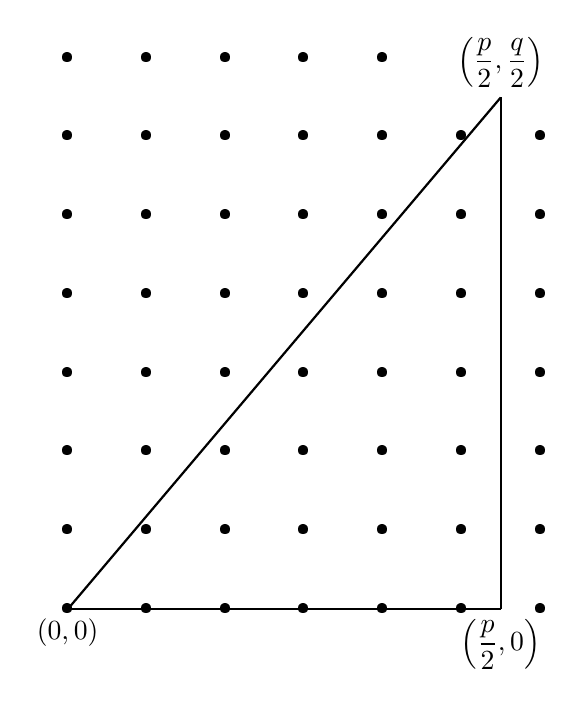
\begin{tikzpicture}
		\draw[thick] (0,0)--(5.5,6.5);
		\draw[thick] (5.5,6.5)--(5.5,0);
		\draw[thick] (0,0)--(5.5,0);
		
		\foreach \Point in {(0,0), (0,1), (0,2), (0,3), (0,4), (0,5), (0,6), (0,7),
			(1,0), (1,1), (1,2), (1,3), (1,4), (1,5), (1,6), (1,7),
			(2,0), (2,1), (2,2), (2,3), (2,4), (2,5), (2,6), (2,7),
			(3,0), (3,1), (3,2), (3,3), (3,4), (3,5), (3,6), (3,7),
			(4,0), (4,1), (4,2), (4,3), (4,4), (4,5), (4,6), (4,7),
			(5,0), (5,1), (5,2), (5,3), (5,4), (5,5), (5,6),
			(6,0), (6,1), (6,2), (6,3), (6,4), (6,5), (6,6)}{
			\node at \Point {\textbullet};
		}
		
		\node [below] at (0,0) {$(0,0)$};
		\node [below] at (5.5,0) {$\displaystyle\left(\frac{p}{2},0\right)$};
		\node [above] at (5.5,6.5) {$\displaystyle\left(\frac{p}{2},\frac{q}{2}\right)$};
		\end{tikzpicture}
	\end{center}
	
	The number of points with integer coordinates inside this triangle equals\[ \sum_{k=1}^{\frac{p-1}{2}} \Big\lfloor\frac{kq}{p} \Big\rfloor.\] You can easily verify this by using the fact that the hypotenuse of triangle lies on the line $y = \frac{q}{p}x$, and so the number of points with $x=k$ (where $1\leq k \leq \frac{p-1}{2}$) inside the triangle equals $\Big\lfloor\frac{kq}{p} \Big\rfloor$ (actually, we are counting the points vertically).
	
	Now consider the triangle with vertices on $(0,0), \left(0,q/2\right)$, and $\left(p/2,q/2\right)$.
	
	\begin{center}
		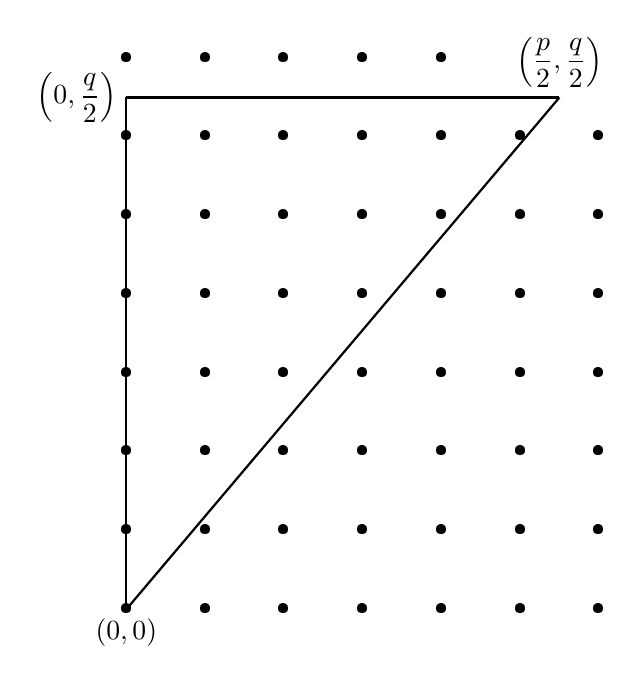
\begin{tikzpicture}
		
		\draw[thick] (0,0)--(5.5,6.5);
		\draw[thick] (5.5,6.5)--(0,6.5);
		\draw[thick] (0,0)--(0,6.5);
		
		\foreach \Point in {(0,0), (0,1), (0,2), (0,3), (0,4), (0,5), (0,6), (0,7),
			(1,0), (1,1), (1,2), (1,3), (1,4), (1,5), (1,6), (1,7),
			(2,0), (2,1), (2,2), (2,3), (2,4), (2,5), (2,6), (2,7),
			(3,0), (3,1), (3,2), (3,3), (3,4), (3,5), (3,6), (3,7),
			(4,0), (4,1), (4,2), (4,3), (4,4), (4,5), (4,6), (4,7),
			(5,0), (5,1), (5,2), (5,3), (5,4), (5,5), (5,6),
			(6,0), (6,1), (6,2), (6,3), (6,4), (6,5), (6,6)}{
			\node at \Point {\textbullet};
		}
		
		\node [below] at (0,0) {$(0,0)$};
		\node [left] at (0,6.5) {$\displaystyle\left(0,\frac{q}{2}\right)$};
		\node [above] at (5.5,6.5) {$\displaystyle\left(\frac{p}{2},\frac{q}{2}\right)$};
		\end{tikzpicture}
	\end{center}
	We can find the number of points with integer coordinates inside this triangle in a similar way to the previous one. This time, count the points horizontally and sum up the number of points with $y=1, y=2, \ldots$, and $y=\frac{p-1}{2}$. The result is \[ \sum_{k=1}^{\frac{q-1}{2}} \Big\lfloor\frac{kp}{q} \Big\rfloor.\]
	
	Now put these two triangles together to form a rectangle with vertices on $(0,0)$, $\left(0,q/2\right)$, $\left(p/2,0\right)$, and $\left(p/2,q/2\right)$.
	
	Let $x$ be number of the points with integer coordinates inside this rectangle. Obviously, $x$ is equal to the sum of such points in triangles (notice that since $p$ and $q$ are different, there is no point with integer coordinates on the hypotenuse of triangles). So
	\begin{align*}
	x = \sum_{k=1}^{\frac{p-1}{2}} \Big\lfloor\frac{kq}{p} \Big\rfloor+ \sum_{k=1}^{\frac{q-1}{2}} \Big\lfloor\frac{kp}{q} \Big\rfloor.
	\end{align*}
	According to lemma \eqref{lem:lawofqrlem2}, it follows that
	\begin{align}\label{eq:qrlawproof1}
	x \equiv \mu(q,p)+\mu(p,q) \pmod 2.
	\end{align}
	Let's count $x$ in another way.
	\begin{center}
		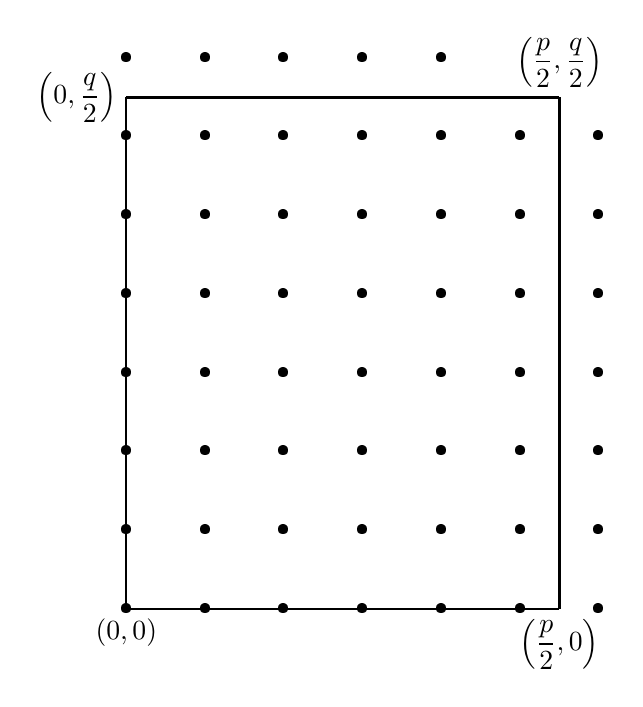
\begin{tikzpicture}
		\draw[thick] (5.5,6.5)--(5.5,0);
		\draw[thick] (0,0)--(5.5,0);
		\draw[thick] (5.5,6.5)--(0,6.5);
		\draw[thick] (0,0)--(0,6.5);
		
		\foreach \Point in {(0,0), (0,1), (0,2), (0,3), (0,4), (0,5), (0,6), (0,7),
			(1,0), (1,1), (1,2), (1,3), (1,4), (1,5), (1,6), (1,7),
			(2,0), (2,1), (2,2), (2,3), (2,4), (2,5), (2,6), (2,7),
			(3,0), (3,1), (3,2), (3,3), (3,4), (3,5), (3,6), (3,7),
			(4,0), (4,1), (4,2), (4,3), (4,4), (4,5), (4,6), (4,7),
			(5,0), (5,1), (5,2), (5,3), (5,4), (5,5), (5,6),
			(6,0), (6,1), (6,2), (6,3), (6,4), (6,5), (6,6)}{
			\node at \Point {\textbullet};
		}
		
		\node [below] at (0,0) {$(0,0)$};
		\node [left] at (0,6.5) {$\displaystyle\left(0,\frac{q}{2}\right)$};
		\node [below] at (5.5,0) {$\displaystyle\left(\frac{p}{2},0\right)$};
		\node [above] at (5.5,6.5) {$\displaystyle\left(\frac{p}{2},\frac{q}{2}\right)$};
		\end{tikzpicture}
	\end{center}
	Clearly, number of points with integer coordinates inside this rectangle is
	\begin{align}\label{eq:qrlawproof2}
	x=\Big\lfloor\frac{p}{2} \Big\rfloor \cdot \Big\lfloor\frac{q}{2} \Big\rfloor = \frac{p-1}{2}\cdot\frac{q-1}{2}.
	\end{align}
	Combining equations \eqref{eq:qrlawproof1} and \eqref{eq:qrlawproof2},
	\begin{align*}
	\mu(q,p)+\mu(p,q) \equiv \frac{p-1}{2}\cdot\frac{q-1}{2} \pmod 2.
	\end{align*}
	Now apply Gauss's criterion to finish the proof:
	\begin{align*}
	\left(\dfrac{p}{q}\right)\left(\dfrac{q}{p}\right) &=(-1)^{\mu(p,q)} \cdot (-1)^{\mu(q,p)} \\
	&= (-1)^{\mu(p,q)+\mu(q,p)}\\
	&=(-1)^{\frac{p-1}{2}\cdot\frac{q-1}{2}}.
	\end{align*}
\end{proof}

\end{document}

\section{Darij-Wolstenholme Theorem}
\documentclass{subfile}

\begin{document}
	The following theorem is a generalization of Wolstenholme's theorem. It was proposed and proved by Darij Grinberg on the \textit{Art of Problem Solving} website. Before stating the theorem, we need to define $v_p(x)$ for a rational number $x$.

	Recall section \eqref{sec:powerofprimes} where we defined $v_p(x)$ for $x$ being an \textit{integer} as the greatest power of $p$ which divides $x$. Now, since we are working with fractions, we need to generalize this concept to include rational numbers.

	\begin{definition}
		Let $p$ be a prime and let $x = \frac{a}{b} \neq 0$ be a rational number reduced to lowest terms. Define the \textit{$p$-adic evaluation of $x$} as $v_p(x) = v_p(a)-v_p(b)$, where $v_p(n)$ is the notation defined in definition \eqref{def:vp}.
	\end{definition}

	\begin{example}
		$v_3\left(\frac{9}{16}\right) = 2$, and $v_5\left(\frac{34}{25}\right) = -2$.
	\end{example}

	\begin{note}
		We can easily check the sign of $v_p(x)$ for any rational number $x=\frac{a}{b}$. If $p\mid a$, then $v_p(x)>0$. If $p$ divides none of $a$ and $b$, then $v_p(x)=0$. And if $p\mid b$, then $v_p(x)<0$. Also,  $ v_{p}\left(xy\right) = v_{p}\left(x\right) + v_{p}\left(y\right)$ and $ v_{p}\left(x + y\right)\geq\min\left(v_{p}\left(x\right),v_{p}\left(y\right)\right)$ for all rationals $x$ and $y$.
	\end{note}

	We can now generalize the concept of congruency to include rational numbers.
	\begin{definition}
		If $x$ and $y$ are two rational numbers such that $ v_{p}\left(x\right)\geq 0$ and $ v_{p}\left(y\right)\geq 0$, then we say that $ x\equiv y\pmod p$ if and only if $ v_{p}\left(x - y\right) > 0$.
	\end{definition}

	The following problem gives you a good sight of the above notation.

	\begin{problem}
		Let $p \geq 3$ be a prime. Prove that $p\mid 2^{p-2}+3^{p-2}+6^{p-2}-1$.
	\end{problem}

	\begin{solution}
		Let $a \bot p$ be an integer. We can write $a^{p-2} \equiv \frac{1}{a} \pmod p$ because
			\begin{align*}
				v_p\left(a^p - \frac{1}{a}\right)=v_p\left(\frac{a^{p-1}-1}{a}\right)>0
			\end{align*}
		by Fermat's little theorem. Now
		\begin{align*}
		2^{p-2}+3^{p-2}+6^{p-2}-1 \equiv \frac{1}{2}+\frac{1}{3}+\frac{1}{6}-1 \equiv 0 \pmod p.
		\end{align*}
	\end{solution}

	\begin{theorem}[Darij-Wolstenholme Theorem]
		Let $p>3$ be a prime and let $u$ be a non-negative and odd integer such that $p \geq u+3$. Then
		\begin{align*}
		v_{p}\left(\sum_{k = 1}^{p - 1}\frac {1}{k^{u}}\right)\geq 2
		\end{align*}
	\end{theorem}

	The idea of the proof is similar to the proof of Wolstenholme's theorem. We need to prove a lemma first.

	\begin{lemma}\label{lem:darijwolstproof}
		Let $p$ be a prime and let $n$ be an integer such that $1 \leq n \leq p-2$. Then
		\begin{align*}
		\sum_{k = 1}^{p - 1} k^n \equiv 0 \pmod p.
		\end{align*}
	\end{lemma}

	\begin{proof}
		There exists an integer $a$ co-prime to $p$ such that $p \nmid a^n -1$. The set $A= \{0, 1^n, 2^n, \ldots, (p-1)^n\}$ forms a compete residue system modulo $p$ (why?). Proposition \eqref{prop:generalcompletesystem} says that the set $B=\{0, a^n, (2a)^n, \ldots, ((p-1)a)^n\}$ also forms a complete residue system modulo $p$. Therefore, the sum of elements of both sets are equivalent modulo $p$. So
		\begin{align*}
			\sum_{k = 1}^{p - 1} k^n
				& \equiv \sum_{k = 1}^{p - 1} (a \cdot k)^n\\
				& \equiv a^n \sum_{k = 1}^{p - 1} k^n \pmod p
		\end{align*}
		This means that
			\begin{align*}
				\left(a^k - 1\right) \sum_{k = 1}^{p - 1} k^n \equiv 0 \pmod p
			\end{align*}
		and since $p \nmid a^n -1$, we should have
			\begin{align*}
				\sum_{k = 1}^{p - 1} k^n \equiv 0 \pmod p.
			\end{align*}
		If the proof seemed confusing to you, here is a potentially better version. Consider a primitive root $g$ of $p$ (we already know there is one from modular arithmetic chapter). Then we also know that $\{1,2,\ldots,p-1\}$ can be generated by $g$ (the set $\{1,g,g^2,\ldots,g^{p-2}\}$). So,
			\begin{align*}
				1^n+2^n+\cdots+(p-1)^n & = 1^n+g^n+g^{2n}+\cdots+\left(g^{p-2}\right)^n\\
										&= \dfrac{(g^n)^{p-1}-1}{g^n-1}\\
										& = \dfrac{g^{(p-1)n}-1}{g^n-1}
			\end{align*}
		From Fermat's little theorem, $g^{p-1}\equiv1\pmod p$, so the conclusion follows.
	\end{proof}

	\begin{proof}[Proof of Darij-Wolstenholme Theorem]
		The idea is to use the trick explained in lemma \eqref{lem:wolstproof1}. That is, we write the given sum as a sum of terms of the form $\frac{1}{k^u}+\frac{1}{(p-k)^u}$. We have
		\begin{align*}
		2\sum_{k = 1}^{p - 1}\frac {1}{k^{u}} &= \sum_{k = 1}^{p - 1}\frac {1}{k^{u}} + \sum_{k = 1}^{p - 1}\frac {1}{\left(p - k\right)^{u}}\\
		&= \sum_{k = 1}^{p - 1}\left(\frac {1}{k^{u}} + \frac {1}{\left(p - k\right)^{u}}\right) \\
		&= \sum_{k = 1}^{p - 1}\frac {k^{u} + \left(p - k\right)^{u}}{k^{u}\left(p - k\right)^{u}}\\
		&=\sum_{k = 1}^{p - 1}\frac {k^{u} + \left(p^{u} - up^{u - 1}k+ \cdots + upk^{u - 1} - k^{u}\right)}{k^{u}\left(p - k\right)^{u}} \\
		&= \sum_{k = 1}^{p - 1}\frac {p^{u} - up^{u - 1}k + \cdots + upk^{u - 1}}{k^{u}\left(p - k\right)^{u}}\\
		&=p \cdot \sum_{k = 1}^{p - 1}\frac {p^{u - 1} - up^{u - 2}k+\cdots + uk^{u - 1}}{k^{u}\left(p - k\right)^{u}}
		\end{align*}
		We have used the fact that $u$ is an odd integer to expand $(p-k)^u$ in above lines. Now since $p>3$ is an odd prime, $v_p(2)=0$ and therefore
			\begin{align*}
				v_{p}\left(2\sum_{k = 1}^{p - 1}\frac {1}{k^{u}}\right)
					&= v_{p}\left(2\right) + v_{p}\left(\sum_{k = 1}^{p - 1}\frac {1}{k^{u}}\right)\\
					& = v_{p}\left(\sum_{k = 1}^{p - 1}\frac {1}{k^{u}}\right)\\
					&=v_{p}\left(p \cdot \sum_{k = 1}^{p - 1}\frac {p^{u - 1} - up^{u - 2}k+\cdots + uk^{u - 1}}{k^{u}\left(p - k\right)^{u}}\right)\\
					&=v_{p}\left(p\right) + v_{p}\left(\sum_{k = 1}^{p - 1}\frac {p^{u - 1} - up^{u - 2}k+\cdots + uk^{u - 1}}{k^{u}\left(p - k\right)^{u}}\right)\\
					&=1+v_{p}\left(\sum_{k = 1}^{p - 1}\frac {p^{u - 1} - up^{u - 2}k+\cdots + uk^{u - 1}}{k^{u}\left(p - k\right)^{u}}\right)
			\end{align*}
		So instead of showing $v_{p}\left(2\sum_{k = 1}^{p - 1}\frac {1}{k^{u}}\right) \geq 2$, it is enough to show that
		\begin{align*}
			v_{p}\left(\sum_{k = 1}^{p - 1}\frac {p^{u - 1} - up^{u - 2}k+\cdots + uk^{u - 1}}{k^{u}\left(p - k\right)^{u}}\right)
				& \geq 1
		\end{align*}
		which is equivalent to showing that
		\begin{align*}
			\sum_{k = 1}^{p - 1}\frac {p^{u - 1} - up^{u - 2}k+\cdots + uk^{u - 1}}{k^{u}\left(p - k\right)^{u}}
				& \equiv 0 \pmod p
		\end{align*}
		Since $p^{u - 1} - up^{u - 2}k+\cdots + uk^{u - 1} \equiv uk^{u - 1} \pmod p$ and $k^{u}\left(p - k\right)^{u} \equiv k^{u}\left( - k\right)^{u} \equiv (-1)^u k^{2u} \pmod p$, we should prove that
			\begin{align*}
				\sum_{k = 1}^{p - 1}\frac {uk^{u - 1}}{\left( - 1\right)^{u}k^{2u}}
					& \equiv\frac {u}{\left( - 1\right)^{u}}\sum_{k = 1}^{p - 1}k^{ - u - 1}\\
					& \equiv 0 \pmod p
			\end{align*}
		From Fermat's little theorem, we have $k^{p-1} \equiv 1 \pmod p$ for every $k$ such that $1 \leq k \leq p-1$. So $ k^{ - u - 1}\equiv k^{ - u - 1}k^{p - 1} = k^{p - u - 2}\pmod p$ and we must prove that
		\begin{align*}
		\frac {u}{\left( - 1\right)^{u}}\sum_{k = 1}^{p - 1}k^{p - u - 2}\equiv 0 \pmod p
		\end{align*}
		which follows directly from lemma \eqref{lem:darijwolstproof} because $ 1\leq p - u - 2\leq p - 2$. The proof is complete.
	\end{proof}

	\begin{problem}
		Let $p>3$ be a prime. Prove that
		\begin{align*}
		\sum_{i = 1}^{\left\lfloor 2p/3\right\rfloor}\frac {\left( - 1\right)^{i - 1}}{i} \equiv 0 \pmod p
		\end{align*}
	\end{problem}

	\begin{solution}
		First, let us prove that
		\begin{align}\label{eq:primefloor}
		p - \left\lfloor \left\lfloor 2p/3\right\rfloor /2\right\rfloor = \left\lfloor 2p/3\right\rfloor + 1
		\end{align}
		where $\lfloor x \rfloor$ is the largest integer not greater than $x$ for any real $x$. Since $p>3$, either $p \equiv 1 \pmod 3$ or $p \equiv 2 \pmod 3$. Consider both cases:
		\begin{itemize}
			\item If $p \equiv 1 \pmod 3$, then $\frac{p-1}{3}$ is an integer and
			\begin{align*}
			2\cdot\frac {p - 1}{3}\leq\frac {2p}{3} < 2\cdot\frac {p - 1}{3} + 1
			\end{align*}
			which means
			\begin{align*}
			\left\lfloor\frac {2p}{3}\right\rfloor &= 2\cdot\frac {p - 1}{3},\\
			\left\lfloor\left\lfloor\frac {2p}{3}\right\rfloor /2\right\rfloor &= \left\lfloor\left(2\cdot\frac {p - 1}{3}\right)/2\right\rfloor = \frac {p - 1}{3}
			\end{align*}
			Finally,
			\begin{align*}
			p - \left\lfloor\left\lfloor\frac {2p}{3}\right\rfloor /2\right\rfloor = p - \frac {p - 1}{3} = 2\cdot\frac {p - 1}{3} + 1 = \left\lfloor\frac {2p}{3}\right\rfloor + 1
			\end{align*}
			as desired.

			\item If $p \equiv 2 \pmod 3$, then $\frac{p-2}{3}$ is an integer and
			\begin{align*}
			2\cdot\frac {p - 2}{3} + 1\leq\frac {2p}{3} < \left(2\cdot\frac {p - 2}{3} + 1\right) + 1
			\end{align*}
			This gives
			\begin{align*}
			\left\lfloor\frac {2p}{3}\right\rfloor
				&= 2\cdot\frac {p - 2}{3} + 1\\
			\left\lfloor\left\lfloor\frac {2p}{3}\right\rfloor /2\right\rfloor
				& =	\left\lfloor\left(2\cdot\frac {p - 2}{3} + 1\right)/2\right\rfloor\\
				& = \left\lfloor\frac {p - 2}{3} + \frac {1}{2}\right\rfloor\\
				& = \frac{p-2}{3}
			\end{align*}
			And finally
				\begin{align*}
					p - \left\lfloor\left\lfloor\frac {2p}{3}\right\rfloor /2\right\rfloor
						& = p - \frac {p - 2}{3}\\
						& = \left(2\cdot\frac {p - 2}{3} + 1\right) + 1\\
						& = \left\lfloor\frac {2p}{3}\right\rfloor + 1
				\end{align*}
		\end{itemize}
		The proof of equation \eqref{eq:primefloor} is finished. We will now prove the problem. Obviously,
			\begin{align*}
				\sum_{i = 1}^{\left\lfloor 2p/3\right\rfloor}\frac {\left( - 1\right)^{i - 1}}{i}
					&= \sum_{\substack{1\leq i\leq \left\lfloor 2p/3\right\rfloor ; \\
						i\text{ is odd}}}\frac {1}{i} + \sum_{\substack{1\leq i\leq \left\lfloor 2p/3\right\rfloor ; \\
						i\text{ is even}}}\frac { - 1}{i} \\
					&= \sum_{\substack{1\leq i\leq \left\lfloor 2p/3\right\rfloor ; \\
							i\text{ is odd}}}\frac {1}{i} - \sum_{\substack{1\leq i\leq \left\lfloor 2p/3\right\rfloor ; \\
							i\text{ is even}}}\frac {1}{i}\\
					&= \left(\sum_{\substack{1\leq i\leq \left\lfloor 2p/3\right\rfloor ; \\
							i\text{ is odd}}}\frac {1}{i} + \sum_{\substack{1\leq i\leq \left\lfloor 2p/3\right\rfloor ; \\
							i\text{ is even}}}\frac {1}{i}\right) - 2\sum_{\substack{1\leq i\leq \left\lfloor 2p/3\right\rfloor ; \\
							i\text{ is even}}}\frac {1}{i} \\
					&= \sum_{i = 1}^{\left\lfloor 2p/3\right\rfloor}\frac {1}{i} - 2\sum_{\substack{1\leq i\leq \left\lfloor 2p/3\right\rfloor ; \\
							i\text{ is even}}}\frac {1}{i}\\
					&= \sum_{i = 1}^{\left\lfloor 2p/3\right\rfloor}\frac {1}{i} - 2\sum_{j = 1}^{\left\lfloor \left\lfloor 2p/3\right\rfloor /2\right\rfloor}\frac {1}{2j} \\
					&= \sum_{i = 1}^{\left\lfloor 2p/3\right\rfloor}\frac {1}{i} + \sum_{j = 1}^{\left\lfloor \left\lfloor 2p/3\right\rfloor /2\right\rfloor}\frac {1}{ - j}\\
					&\equiv\sum_{i = 1}^{\left\lfloor 2p/3\right\rfloor}\frac {1}{i} + \sum_{j = 1}^{\left\lfloor \left\lfloor 2p/3\right\rfloor /2\right\rfloor}\frac {1}{p - j} \pmod p
			\end{align*}
		In the second sum in the last line of above equations, we have used the fact that $-j \equiv p-j \pmod p$. Replacing $ j$ by $ p - i$ in the second sum, we have
		\begin{align*}
		\sum_{i = 1}^{\left\lfloor 2p/3\right\rfloor}\frac {\left( - 1\right)^{i - 1}}{i} &\equiv \sum_{i = 1}^{\left\lfloor 2p/3\right\rfloor}\frac {1}{i} + \sum_{i = p - \left\lfloor \left\lfloor 2p/3\right\rfloor /2\right\rfloor}^{p - 1}\frac {1}{i}
		\end{align*}
		Using \eqref{eq:primefloor}, we can write $i = p - \left\lfloor \left\lfloor 2p/3\right\rfloor /2\right\rfloor = \left\lfloor 2p/3\right\rfloor + 1$ and so by Wolstenholme's theorem,
		\begin{align*}
		\sum_{i = 1}^{\left\lfloor 2p/3\right\rfloor}\frac {\left( - 1\right)^{i - 1}}{i}  &\equiv \sum_{i = 1}^{\left\lfloor 2p/3\right\rfloor}\frac {1}{i} + \sum_{i = \left\lfloor 2p/3\right\rfloor + 1}^{p - 1}\frac {1}{i}\\
		&\equiv \sum_{i = 1}^{p - 1}\frac {1}{i}\pmod p\\
		&\equiv 0 \pmod p
		\end{align*}
		This finishes the proof of the problem.
	\end{solution}
\end{document}

\section{Generalization of Wilson's and Lucas' Theorem}\label{sec:wilsongeneral}
\documentclass{subfile}

\begin{document}
Wilson's theorem says that $(p-1)! \equiv -1 \pmod p$ for all primes $p$. Clearly, for any integer $n$ larger than $p$, we have $n! \equiv 0 \pmod p$. Now, if we remove the multiples of $p$ from $n!$ and then calculate the result modulo $p$, what would it be? We will state this as a generalization for Wilson's theorem. But first, some definitions and lemmas.

	\begin{definition}
		Let $n$ be a positive integer and $p$ a prime number. The \textit{$p$-reduced factorial of $n$} is the product of all positive integers less than or equal to $n$ which are not divisible by $p$. We denote this by $(n!)_p$.
	\end{definition}

	\begin{example}
		The $5$-reduced factorial of $10$, $(10!)_5$, is
			\begin{align*}
				(10!)_5
					& = 9 \times 8 \times 7 \times 6 \times 4 \times 3 \times 2 \times 1\\
					& = 72,576
			\end{align*}
	\end{example}


	\begin{theorem}\label{thm:reducedfactorialmodp}
		Let $p$ be a prime number and let $(n_k n_{k-1}\cdots n_1 n_0)_p$ be a positive integer. Then
			\begin{align*}
				(n!)_p
					& \equiv (-1)^{\left[\frac{n}{p}\right]} \cdot n_0!\pmod p
			\end{align*}
	\end{theorem}

	\begin{proof}
		The numbers not divisible by $p$ among $1, 2, \cdots, n$ are
			\[\begin{array}{*{20}{c}}
				1&2& \cdots &{{n_0}}& \cdots &{p - 1}\\
				{p + 1}&{p + 2}& \cdots &{p + {n_0}}& \cdots &{2p - 1}\\
				\vdots & \vdots & \ddots & \vdots & \ddots & \vdots \\
				{( {[\frac{n}{p}] - 1} )p + 1}&{( {[\frac{n}{p}] - 1} )p + 2}& \cdots &{( {[\frac{n}{p}]p - 1} )p + {n_0}}& \cdots &{[\frac{n}{p}]p - 1}\\
				{[\frac{n}{p}]p + 1}&{[\frac{n}{p}]p + 2}& \cdots &{[\frac{n}{p}]p + {n_0}}&{}&{}
			\end{array}\]

	Product of these numbers, $(n!)_p$ is
		\begin{align*}
			\left(\prod_{k=0}^{[\frac np]-1}\!\!\left((kp+1)\cdot(kp+2)\cdots(kp+p-1)\right)\right)  \cdot
			\left([\tfrac np]p+1\right)\left([\tfrac np]p+2\right)\dots\left([\tfrac np]p+n_0\right)
		\end{align*}
	which is equal to
		\begin{align*}
			\left(\prod_{k=0}^{[\frac np]-1}\!\!\left(1\cdot2\cdots(p-1)\right)\right)  \cdot
			\left([\tfrac np]p+1\right)\left([\tfrac np]p+2\right)\dots\left([\tfrac np]p+n_0\right)
				& \equiv \left(\prod_{k=0}^{[\frac np]-1}\!\!\left(-1\right) \right) \cdot \left(
				1 \cdot 2 \cdots n_0\right)\\
				& \equiv(-1)^{[\frac np]} n_0!\pmod p
		\end{align*}
	\end{proof}


	\begin{proposition}
		Let $p\geq 3$ be a prime and $n$ be a positive integer. Then
			\begin{align*}
				(p^n!)_p \equiv -1 \pmod{p^n}
			\end{align*}
	\end{proposition}

	\begin{proof}
		This is exactly the same as the proof of Wilson's theorem. All numbers in the product $(p^n!)_p$ have a multiplicative inverse modulo $p^n$. If the inverse of a number $a$ among these numbers is $b \neq a$, then $a b \equiv 1 \pmod{p^n}$ and we can remove $a$ and $b$ from the product $(p^n!)_p$. Our only concern is when the inverse of $a$ equals $a$ itself. But if that's the case, we have
			\begin{align*}
				a^2
					& \equiv 1 \pmod{p^n}\\
				\implies p^n
					& \mid (a-1)(a+1)
			\end{align*}
		But since $(a-1,a+1)=2$, we should have $a \equiv \pm 1 \pmod{p^n}$, which means $a$ is either $1$ or $p^n-1$. All in all, we see that the product of all numbers in $(p^n!)_p$ except $p^n-1$ equals $1$ modulo $p^n$, and if we multiply this number by $p^n-1$, the result will be $-1$ modulo $p^n$.
	\end{proof}

	\begin{problem}
		Prove that $(2^n!)_2 \equiv 1 \pmod{2^n}$.
	\end{problem}

We are ready to prove the following theorem.

	\begin{theorem}[Generalization of Wilson's Theorem]\label{thm:wilsongeneral}
		Let $p$ be a prime number and let $(n_k n_{k-1}\cdots n_1 n_0)_p$ be the representation of a positive integer $n$ in base $p$. Then
			\begin{align}\label{eq:wilsongeneral}
				\dfrac{n!}{p^{v_p(n!)}}\equiv (-1)^{v_p(n!)} n_0!n_1!\dots n_k!\pmod p
			\end{align}
	\end{theorem}

	\begin{proof}
		According to theorem \eqref{thm:reducedfactorialmodp}, one can write
			\begin{align*}
				n!
					& = (n!)_p \cdot p^{\left\lfloor n/p\right\rfloor}\left(\left\lfloor\frac{n}{p}\right\rfloor\right)!\\
					& \equiv (-1)^{\lfloor n/p\rfloor} n_0! \cdot p^{\lfloor n/p \rfloor}\left(\left\lfloor\frac{n}{p}\right\rfloor\right)!
			\end{align*}
		Now write $(\lfloor \frac np\rfloor)!$ in the same way and continue this process. The result is concluded.
	\end{proof}

	\begin{note}
		If you are interested, you can find a (different) generalization of Wilson's theorem in Problem \ref{thm:genWilson}.
	\end{note}
	\begin{theorem}[Generalization of Lucas' Theorem]
		Let $p$ be a prime number and $m, n$, and $r$ be non-negative integers such that $r=m-n$ and
			\begin{align*}
				m&=m_kp^k+m_{k-1}p^{k-1}+\cdots +m_1p+m_0\\
				n&=k_kp^k+n_{k-1}p^{k-1}+\cdots +n_1p+n_0\\
				r&=r_kp^k+r_{k-1}p^{k-1}+\cdots +r_1p+r_0
			\end{align*}
		Also, let $\ell = v_p\left(\binom{m}{n}\right)$. Then
			\begin{align*}
				\frac1{p^\ell}\binom{m}{n}\equiv (-1)^\ell
				\left(\frac{m_0!}{n_0!r_0!}\right) \left(\frac{m_1!}{n_1!r_1!}\right) \dots \left(\frac{m_d!}{n_d!r_d!}\right) \pmod p
			\end{align*}
	\end{theorem}

	\begin{proof}
		Note that
			\begin{align*}
				\ell
					&= v_p\left(\binom{m}{n}\right) = v_p\left(\frac{m!}{n!r!}\right) = v_p(n!)-v_p(n!)-v_p(r!)\\
					&=\sum_{i=1}^{k}\left\lfloor\dfrac{m}{p^i}\right\rfloor - \sum_{i=1}^{k}\left\lfloor\dfrac{n}{p^i}\right\rfloor -\sum_{i=1}^{k}\left\lfloor\dfrac{r}{p^i}\right\rfloor\\
					&=\sum_{i=1}^{k}\left(\left\lfloor\dfrac{m}{p^i}\right\rfloor - \left\lfloor\dfrac{n}{p^i}\right\rfloor - \left\lfloor\dfrac{r}{p^i}\right\rfloor \right)
			\end{align*}
		Just like the proof of theorem \eqref{thm:wilsongeneral}, we can write
			\begin{align*}
				\binom {m}{n}
					& =\frac{(m!)_p}{(n!)_p (r!)_p}\cdot
				\frac{p^{\lfloor m/p\rfloor}}{p^{\lfloor n/p\rfloor} \cdot p^{\lfloor r/p\rfloor}}\cdot
				\frac{\left\lfloor\dfrac{m}{p}\right\rfloor!}{\left\lfloor\dfrac{n}{p}\right\rfloor! \cdot \left\lfloor\dfrac{r}{p}\right\rfloor!}
			\end{align*}
		Use induction and generalization of Wilson's theorem to finish the proof.
	\end{proof}


\end{document}

\section{Inverse of Euler's Totient Function}
\documentclass{subfile}

\begin{document}
	For a given positive integer $n$, we can find $\varphi(n)$ after factorizing $n$. What about the reverse problem? That is, given $\varphi(n)$, can you find $n$? A more interesting question is whether this solution $n$ is unique or there are other solutions. We can answer the latter question pretty quickly using an example: $\varphi(4)=2$ and $\varphi (6)=2$. In other words, $\varphi $ is not a one to one function. Now, another question normally arises here:
		\begin{problem}
			Is there any $n\in\mathbb{N}$ such that $\varphi(x)=n$ has a unique solution for $x$?
		\end{problem}
	There are good results on this topic. It has also been studied how to find such $x$, and the upper or lower bounds of $x$. Here we will discuss some of the results, which fits into our book.
		\begin{definition}[Inverse Phi]
			Let $n$ be a positive integer. Assume that $\varphi ^{-1}(n)$ is the \textit{set} of all possible values of $x\in\mathbb{N} $ such that $\varphi (x)=n$. In other words,
				\begin{align*}
					\varphi^{-1}(n) & = \{x:\varphi(x)=n\}.
				\end{align*}
			We call $\varphi^{-1}(n)$ the \textit{inverse of Euler's totient function}, or simply the \textit{inverse of phi function}. Moreover, for ever positive integer $x$, we define $N(x)$ to be the number of positive integers $y$ such that $\varphi(x)=\varphi(y)$.
		\end{definition}
	
	Carmichael stated in \cite{carmichael} that the cardinality (number of elements) of $\varphi^{-1}(n)$ is always greater than $1$ but due to his proof being inadequate, this is a conjecture now:
		\begin{conjecture}[Carmichael's Totient Conjecture]
			For a positive integer $n$, the number of solutions to $\varphi(x)=n$ is either $0$ or at least $2$.
		\end{conjecture}
	After this statement, quite a lot of number theorists worked on it. There has been no proof of the theorem to our knowledge, though there are some nice results on it. And it is indeed a very interesting topic to work on. Even though it is a conjecture, everything points this to be true. For example, \textit{Klee} pointed out in \cite{klee} that if $N(x)=1$ then $x$ and $\varphi(x)$ are both larger than $10^{400}$. Carmichael originally proved that $x>10^{37}$ must be true. Let's start investigating $N(x)$.
		\begin{theorem}\slshape
			Let $x$ be a positive integer. If $N(x)=1$, then $x$ is divisible by $4$.
		\end{theorem}
		
		\begin{proof}
			For $n>2$, $\varphi(n)$ is always even. If $x$ is odd, then $2\bot x$ so $\varphi(2x)=\varphi(x)$ so $y=2x$ is a solution, so contradiction. Again, if $x=2t$ with $t$ odd then $\varphi(x)=\varphi(t)$ by same argument. Thus, $x$ is divisible by $4$.
		\end{proof}
	The following theorem is due to Carmichael.
	
		\begin{theorem} \slshape
			Let $x$ be a positive integer and let $p=2^k+1$ be a prime divisor of $x$, where $k$ is some natural number. If $N(x)=1$, then $p^2|x$.
		\end{theorem}
		
		\begin{proof}
			To the contrary, assume that $x=2^eps$ for some positive integers $e$ and $s$ with $s\bot 2p$. Then,
				\begin{align*}
					\varphi(x)  & = \varphi(2^e)\varphi(p)\varphi(s)\\
							& = 2^{e-1}2^k\varphi(s)\\
							& = \varphi(2^{k+e})\varphi(s)\\
							& = \varphi(2^{k+e}s).
				\end{align*}
			Thus, $y=2^{k+e}s\neq x$ satisfies the condition, so we must have $p|s$ and hence $p^2 | x$.
		\end{proof}
	Here is a very nice result that provides us with a sufficient condition for $N(x)=1$ to happen.. The result is due to C. Pomerance \cite{pomerance}.
		\begin{theorem}[Carl Pomerance]\slshape
			 Let $x$ be a positive integer. Suppose that the following property holds for every prime $p$:
				\begin{align*}
					p-1|\varphi(x)& \text{ implies } p^2|x.
				\end{align*}
			Then $N(x)=1$. That is, if $\varphi(y)=\varphi(x)$ for some positive integer $y$, then $y=x$.
		\end{theorem}
		
		\begin{proof}
			For every positive integer $n$, define $S(n)$ to be the set of prime divisors of $n$. If the prime factorization of $n$ is $\prod_{i=1}^{r}p_i^{e_i}$, then
				\begin{align*}
					\varphi(n) & = \prod_{i=1}^{r}p_i^{e_i-1}(p_i-1).
				\end{align*}
			According to our assumption, $x$ is a positive integer such that if $p-1|\varphi(x)$ then $p^2|x$. We are required to prove that under this assumption, if $\varphi(x)=\varphi(y)$ then $x=y$ must hold. If $p\in S(y)$ then $p-1|\varphi(y)=\varphi(x)$. So, from the assumption, $p^2|x$ for any prime $p$ in $S(y)$. This gives us $S(y)\subseteq S(x)$.
				
			We will investigate the exponent of a prime $p$ in $\varphi(n)$. There are two cases:
				\begin{enumerate}
					\item $p$ divides $n$. Suppose that $p^e\|n$. Then we have $p^{e-1}|\varphi(n)$. But is this the highest exponent possible? No. Because in the factorization of $\varphi(n)$, there are factors of the form $(q-1)$ for any other prime divisor $q$ of $n$. If $p|q-1$ for any such $q$, those will contribute to $v_p(\varphi(n))$ as well. That is,
						\begin{align*}
							v_p(\varphi(n)) & = v_p(n)-1+\sum_{q\in S(n)}v_p(q-1).
						\end{align*}
					
					\item $p$ does not divide $n$. In this case, only factors of the form $(q-1)$ for any prime divisor $q$ of $n$ may contribute to $v_p(\varphi(n))$. In other words,
						\begin{align*}
							v_p(\varphi(n)) & = \sum_{q\in S(n)}v_p(q-1).
						\end{align*}
				\end{enumerate}

			Combining these two results, we find out that for any prime $p$ and any positive integer $n$,
				\begin{align*}
					v_p(\varphi(n)) & = 
						\begin{cases}
							\displaystyle\sum_{q\in S(n)}v_p(q-1),&\text{ if }p\nmid n,\\
							v_p(n)-1+\displaystyle \sum_{q\in S(n)}v_p(q-1),&\text{ otherwise}.
						\end{cases}
				\end{align*}
			Let $p$ be a prime factor of $x$. Since $\varphi(x)=\varphi(y)$, for any prime $p$, we must have
				\begin{align*}
					v_p(\varphi(x)) & = v_p(\varphi(y)).
				\end{align*}
			There are two cases to consider.
				\begin{enumerate}[1.]
					\item $p\notin S(y)$ or $p\nmid y$. Then,
							\begin{align*}
								v_p(x)-1+\sum_{q\in S(x)}v_p(q-1) & = \sum_{q\in S(y)}v_p(q-1)\\
																	  & \leq\sum_{q\in S(x)}v_p(q-1) \quad \text{ since }S(y)\subseteq S(x).
							\end{align*}
						The latter result implies $v_p(x) \leq 1.$ But this is impossible since $v_p(x)\geq2$ due to the fact that $p^2|x$.
					\item $p\in S(y)$. That is, $p|y$, or $S(x)=S(y)$. In this case we should expect to get $x=y$. One way to prove this is to show that $v_p(x)=v_p(y)$. Notice that
						\begin{align*}
							v_p(x) & = v_p(\varphi(x))+1-\sum_{q\in S(x)} v_p(q-1)\\
									 & = v_p(\varphi(y))+1-\sum_{q\in S(y)} v_p(q-1)\quad \text{ since }\varphi(x)=\varphi(y)\text{ and }S(x)=S(y)\\
									 & = v_p(y),
						\end{align*}
				\end{enumerate}
			which was what we wanted.
		\end{proof}
	
	Gupta \cite{gupta} found upper and lower bounds for $\varphi^{-1}(n)$. For odd $n$, $\varphi^{-1}(n)$ is empty. Therefore, we only need to consider the case when $n$ is even. 
		\begin{theorem}[Gupta]\slshape\label{thm:gupta}
			Let $m$ and $n$ be two positive integers such that $n\in\varphi^{-1}(m)$. Then,
				\begin{align*}
					m < n & \leq m\prod_{p-1|m}\dfrac{p}{p-1}.
				\end{align*}
		\end{theorem}
		
		\begin{proof}
			For even $n$, $m=\varphi(n)<n$ because $\varphi(n)=n$ holds for $n=1$ only. This proves the lower bound. For the upper bound, we can write
				\begin{align*}
					\dfrac{n}{\varphi(n)} & = \prod_{p|n}\dfrac{p}{p-1}\\
									  & \leq \prod_{p-1|m}\dfrac{p}{p-1}.
				\end{align*}
			The last line is true because if $p|n$ then $p-1|m$ must hold, but the converse is not true. If $p-1|m$, $p$ may or may not divide $n$.
		\end{proof}
	
	Now we will look at the elements of $\varphi^{-1}(m)$.
		\begin{theorem}\slshape
			Let $m$ be a positive integers and suppose that $\varphi^{-1}(m)$ contains $A$ elements. Then, the number of odd elements of $\varphi^{-1}(m)$ is less than or equal to $A/2$.
		\end{theorem}
		
		\begin{proof}
			For a positive integer $n$, if $\varphi(n)=m$ then $\varphi(2n)=m$ is true as well. Thus, for any odd $n$, there is an even $x$ which belongs to $\varphi^{-1}(m)$. This proves that the number of odd elements is at most half of the number of elements in $\varphi^{-1}(m)$.
		\end{proof}
		
		\begin{theorem}\slshape
			For a prime $p$, there exists a positive integer $n$ such that $n\in\varphi^{-1}(2p)$ if and only if $2p+1$ is a prime.
		\end{theorem}
		
		\begin{proof}
			The ``only if'' part is easy to prove. When $q=2p+1$ is a prime, $\varphi(q)=2p$ so $q\in\varphi^{-1}(2p)$.
			
			Now we prove the ``if'' part. For a positive integer $n\in\varphi^{-1}(m)$, consider that $\varphi(n)=2p$. In other words, suppose that $n \in\varphi^{-1}(2p)$.  If $p=2$ we see that $n=5$ works. We need to show it for odd $p$ now.
			
			Suppose that $n= 2^a p_1^{e_1}p_2^{e_2}\dots p_k^{e_k}$, where $p_1, p_2, \dots, p_k$ are odd primes. Obviously, both $a$ and $k$ cannot be zero at the same time. We have three cases here:
			
				\begin{enumerate}
					\item If $a$ and $k$ are both non-zero, then
						\begin{align*}
							\varphi(n) &= 2^{a-1} p_1^{e_1-1}p_2^{e_2-1}\dots p_k^{e_k-1} (p_1-1)(p_2-1)\dots (p_k-1)\\
									   &= 2p.
						\end{align*}
					Notice that $v_2(\varphi(n)) \geq a-1+k$ and $v_2(2p)=1$. Therefore, $a+k-1 \leq 1$ or $a+k \leq 2$. This gives $a=k=1$, which means $n=2p_1$. Then,
						\begin{align*}
							\varphi(n)   &= p_1-1\\
									     &= 2p\\
							\implies p_1 &= 2p+1,
						\end{align*}
					implying $2p+1$ is a prime.
					
					\item If $a=0$, then
						\begin{align*}
							\varphi(n) &= p_1^{e_1-1}p_2^{e_2-1}\dots p_k^{e_k-1} (p_1-1)(p_2-1)\dots (p_k-1)\\
									   &= 2p.
						\end{align*}
					In this case, $1 = v_2(2p) = v_2(\varphi(n)) \geq k$, and hence $k=1$ or $n=p_1$. So, $\varphi(n)=p_1-1=2p$, and $2p+1$ will be a prime in this case.
					
					\item If $k=0$, then
						\begin{align*}
							\varphi(n) &= 2^{a-1}\\
									   &= 2p,
						\end{align*}
					which is not possible.
				\end{enumerate}
			The proof is complete.
		\end{proof}
	
	We leave the following theorems as exercise for the reader.
		\begin{theorem}\slshape
			The number of odd elements in $\varphi^{-1}(2^k)$ is $0$ or $1$.
		\end{theorem}
		
		\begin{theorem}\slshape
			For an odd $m$, the number of odd elements in $\varphi^{-1}(m)$ is equal to the number of even elements.
		\end{theorem}
	

\end{document}

\newpage
\section{Exercises}
%Thue
\begin{problem} %https://artofproblemsolving.com/community/c6h552600
	Let $p$ be a prime number. Prove that there exist integers $x$ and $y$ such that $p=2x^2+3y^2$ if and only if $p$ is congruent to $5$ or $11$ modulo $24$.
\end{problem}

%	\begin{solution}
%		The $\rightarrow$ part is obvious with quadratic residues modulo $24$ so let me prove the $\leftarrow$ part.
%
%		One can easily calculate $\left(\frac{\frac{p-3}{2}}{p}\right)$ for the cases $p\equiv 5\mod 24$ or $p\equiv 11\mod 24$. It equals $1$ hence there exist an integer $a$ such that $a^2\equiv \frac{p-3}{2}\mod p$ or $2a^2\equiv -3\mod p$. Consider the set of integers of the form $ax-y$ where $0\le x,y< \sqrt{p}$. The number of possible pairs $(x,y)$ is then greater than $p$, so by pigenhole principle , there exist integers $0\le x_1,y_1,x_2,y_2<\sqrt{p}$ such that $ax_1-y_1\equiv ax_2-y_2\mod p$ which implies $ax\equiv y\mod p$ where $x_1-x_2=x$ and $y_1-y_2=y$. Thus $a^2x^2\equiv y^2\mod p$ or $-3x^2\equiv 2y^2\mod p\implies 3x^2+2y^2\equiv 0\mod p$. Since $0<x^2,y^2<p$ , we have $4$ possible cases :
%
%		$1)3x^2+2y^2=p$: Then the desired result follows.
%
%		$2)3x^2+2y^2=2p$: Since $x$ is even write $x=2x_1$ to get $6x_1^2+y^2=p$ which contradicts $p$ being congruent to $-1$ modulo $6$.
%
%		$3)3x^2+2y^2=3p$: Since $y$ is a multiple of $3$ write $y=3y_1$ to get $x^2+6y_1^2=p$, again same contradiction.
%
%		$4)3x^2+2y^2=4p$: Since $x$ is even write $x=2x_1$ to get $6x_1^2+y^2=2p$. Since $y$ is even write $y=2y_1$ to get $3x_1^2+2y_1^2=p$ so the desired result follows.
%	\end{solution}

\begin{problem}[K$\ddot{\mbox{o}}$MaL] %http://www.komal.hu/verseny/feladat.cgi?a=feladat&f=A618&l=en
	Prove that the equation $x^3-x+9=5y^2$ has no solution among the integers.
\end{problem}

\begin{problem}[India 1998]
	If an integer $n$ is such that $7n$ is the form $a^2 + 3b^2$, prove that $n$ is also of that form.
\end{problem}

\begin{problem}[USA TST 2017] %https://artofproblemsolving.com/community/c6h1388623
	Prove that there are infinitely many triples $(a, b, p)$ of positive integers with $p$ prime, $a < p$, and $b < p$, such that $(a + b)^p - a^p - b^p$ is a multiple of $p^3$.
\end{problem}

\begin{problem}
	Let $p$ be a prime other than $7$. Prove that the following conditions are equivalent:
	\begin{enumerate}
		\item There exist integers $x$ and $y$ such that $x^2+7y^2=p$.
		\item $\left(\dfrac{-7}{p}\right) = 1$.
		\item $p$ is congruent to $1,2$, or $4$ modulo $7$.
	\end{enumerate}
\end{problem}

\begin{problem}
	Let $p$ be a prime larger than $5$. Prove that the following conditions are equivalent:
	\begin{enumerate}
		\item There exist integers $x$ and $y$ such that $x^2+6y^2=p$.
		\item $p$ is congruent to $1$ or $7$ modulo $24$.
	\end{enumerate}
\end{problem}

\begin{problem}[Vietnam TST 1998] %https://artofproblemsolving.com/community/c6h42389
	Let $d$ be a positive divisor of $5 + 1998^{1998}$. Prove that $d = 2 \cdot x^2 + 2 \cdot x \cdot y + 3 \cdot y^2$, where $x, y$ are integers if and only if $d$ is congruent to 3 or 7 $\pmod{20}$.
\end{problem}

%	\begin{solution}
%		First note that $gcd(3,d)=gcd(2,d)=1$
%		Let $1998^{999}=a$. Then by Thue's lemma we have $a^2x^2 \equiv y^2(mod$ $d)$ for some positive integers $x,y\le \sqrt{d}$
%
%		And since $a^2\equiv -5(mod$ $d)$ then $a^2x^2\equiv -5x^2\equiv y^2(mod$ $d)$
%		So $5x^2+y^2$ is divisible by $d$ and since $x,y\le \sqrt{d}$ then all posible cases are $k=5x^2+y^2:=d,2d,3d,4d,5d,6d$
%
%		$A)$ If we have $d\equiv 3,7(mod$ $20)$ then $k$ cannot be $d,4d,5d,6d$
%		So we must have $5x^2+y^2=2d$ or $3d$.
%		$1)$ When $5x^2+y^2=2d$ and since $d$ is odd then $x,y$ must have same parity.
%		So we have $y=x+2s$ for some integer $s$ and $d=2xs+2s^2+3x^2$ q.e.d
%		$2)$ When $5x^2+y^2=3d$ and since $gcd(3,d)=1$ then we must have $y-x=3t$ or $y+x=3t$ for some integer $t$.
%		If $y-x=3t$ then $d=2x^2+2xt+3t^2$
%		If $y+x=3t$ then $d=2x^2+2xr+3r^2$ where $r=-t$
%		q.e.d
%		$B)$ If $d=2x^2+2xy+3y^2$ then we must have $d\equiv 3,7(mod$ $20)$ which is easy to prove.
%	\end{solution}

\begin{problem}[Romania TST 1997] %https://artofproblemsolving.com/community/c146h150923
	Let $A$ be the set of positive integers of the form $a^2 +2b^2$, where $a$ and $b$ are integers and $b \neq 0$. Show that if $p$ is a prime number and $p^2 \in A$, then $p \in A$.
\end{problem}

%	\begin{solution}
%		Suppose that $ p^{2}\in A$. Write $ p^{2}= a^{2}+2b^{2}$ for some positive integers $ a$ and $ b$. Reading the equation modulo $ p$ yields $ a^{2}\equiv-2 b^{2}\; (mod\; p)$. Multiplying the inverse of $ b$ modulo $ p$,\footnote{ It's clear that $ b < p$ so that $ b$ is not divisible $ p$.} we get
%		\[ \left( a b^{-1}\right)^{2}\equiv-2\; (mod\; p).\]
%		Taking $ \alpha\equiv a b^{-1}\; (mod\; p)$ in Thue's Lemma, we can find a pair $ (m,n)$ of integers satisfying that $ n\equiv\alpha m\; (mod\; p)$ and $ 0 <\vert m\vert ,\vert n\vert <\sqrt{p}$. After squaring the congruence, we have
%		\[ n^{2}\equiv{\alpha}^{2}{m}^{2}\equiv-2m^{2}\; (mod\; p).\]
%		In other words, $ n^{2}+2m^{2}$ is divisible by $ p$. Since $ 0 <\vert m\vert ,\vert n\vert <\sqrt{p}$ or since $ 0 < n^{2}+2m^{2}< 3p$, this means that $ n^{2}+2m^{2}$ is $ p$ or $ 2p$. In case when $ p = n^{2}+2m^{2}$, it is clear that $ p\in A$. In case when $ 2p = n^{2}+2m^{2}$, we see that $ n$ is even so that $ p = m^{2}+2\left(\frac{n}{2}\right)^{2}\in A$.
%	\end{solution}

%Chicken McNugget

\begin{problem}[India TST 2003]
	On the real number line, paint red all points that correspond to integers of the form $81x+100y$, where $x$ and $y$ are positive integers. Paint the remaining integer point blue. Find a point $P$ on the line such that, for every integer point $T$, the reflection of $T$ with respect to $P$ is an integer point of a different color than $T$.
\end{problem}

\begin{problem}[USAMO 2001]
	Let $S$ be a set of integers (not necessarily positive) such that
		\begin{enumerate}
			\item there exist $a,b \in S$ with $\gcd(a,b)=\gcd(a-2,b-2)=1$;
			\item if $x$ and $y$ are elements of $S$ (possibly equal), then $x^2-y$ also belongs to $S$.
		\end{enumerate}
	Prove that $S$ is the set of all integers.
\end{problem}

%Vietta Jumping

\begin{problem} %https://artofproblemsolving.com/community/c6h349211
	Let $a, b$, and $n$ be positive integers such that $n>2$. Prove that if
		\begin{align*}
			k = \frac{a^n+b^n}{(ab)^{n-1}+1}
		\end{align*}
	is an integer, then $k$ is a perfect $n^{th}$ power.
\end{problem}

%	\begin{solution}
%		We have $ a = b, \; k=\displaystyle{\frac{a^n+b^n}{(ab)^{n-1}+1}} \in \mathbb{N}^+ \Rightarrow a=b=k=1=1^n$
%		Now assume that $a,b,k,n \in \mathbb{N}^+, \; a<b,\;n>1,\; a^n-k=(ka^{n-1}-b)b^{n-1}$
%		(1) If $k > a^n$ then $k > k-a^n = b^{n-1} (b-ka^{n-1}) \ge b^{n-1}$
%		$\quad \quad$ thus $b > ka^{n-1} \ge k > b^{n-1}$. which cannot happen.
%		(2) If $k < a^n$, then $ka^{n-1}-b = \displaystyle{\frac{a^n-k}{b^{n-1}}} < a$, $ka^{n-1} < a+b$, $(k-1)a^{n-1} < a+b - a^{n-1} \le b$
%		Thus $k > 1 \Rightarrow a^{n-1} \le (k-1)a^{n-1} < b \Rightarrow a^n-k = (ka^{n-1}-b)b^{n-1} \ge b^{n-1} >$ $ (a^{n-1})^{n-1} \ge a^n$,
%		that's wrong and so $k=1=1^n$
%		(3) If $k = a^n$ then $b=ka^{n-1}=a^{2n-1} \; b^n = a^{2n^2-n} = a^{2n(n-1) + n}$ hence $\displaystyle{\frac{a^n+b^n}{(ab)^{n-1}+1}=\frac{a^n(1+a^{2n(n-1)})}{(a^{2n})^{n-1}+1}} = a^n$
%	\end{solution}

\begin{problem}[IZHO 2005] %https://artofproblemsolving.com/community/c6h1351952
	Solve the equation  $ p^2 - 6pq + (q^2 + 4) = 0$ in prime numbers less than $2005$.
\end{problem}

\begin{problem}
	Let $ a,b$, and $k $ be positive integers such that
		\begin{align*}
			k=\frac{a^2+b^2}{ab-1}
		\end{align*}
	Prove that $ k=5 $.
\end{problem}

\begin{problem}[IMO 2007] %https://artofproblemsolving.com/community/c6h159987
	Let $a$ and $b$ be positive integers. Show that if $4ab - 1$ divides $(4a^{2} - 1)^{2}$, then $a = b$.
\end{problem}

\begin{problem}[PEN] %https://artofproblemsolving.com/community/c146h150372
	If $a, b, c$ are positive integers such that \[0 < a^{2}+b^{2}-abc \le c\] show that $a^{2}+b^{2}-abc$ is a perfect square.
\end{problem}

\begin{problem}[IMO ShortList 2003] %https://artofproblemsolving.com/community/c6h94
	Determine all pairs of positive integers $(a,b)$ such that \[ \dfrac{a^2}{2ab^2-b^3+1} \] is a positive integer.
\end{problem}

\begin{problem} %https://artofproblemsolving.com/community/c6h1320685
	Find all triples $(x,y,z)$ of positive integers such that $(x+y+z)^2=7xyz$.
\end{problem}

\begin{problem} %https://artofproblemsolving.com/community/c6h417499
 Let $a$ and $b$ be positive integers such that $ab$ divides $a^2 + b^2 + 2$. Prove that $\frac{a^2 + b^2 + 2}{ab} = 4$.
\end{problem}

\begin{problem} %https://artofproblemsolving.com/community/c6h408739
	Find all positive integers $x,y$, and $z$ such that $x^2+y^2+2=xyz$.
\end{problem}

\begin{problem}[Ireland 2005] %https://artofproblemsolving.com/community/c6h560119
	Let $m,n$ be integers with the same parity such that $m^2-n^2+1$ divides $n^2-1$. Prove that $m^2-n^2+1$ is a perfect square.
\end{problem}

\begin{problem}[Mongolia 2000] %https://artofproblemsolving.com/community/c6h2782
	For which positive integer $k$ there exist positive integers $x,y$, and $z$ such that $(x+y+z)^2= kxyz$?
\end{problem}

\begin{problem} %https://artofproblemsolving.com/community/c146h459442
	Prove that the following equation has no positive integer solution $(x,y,z)$ \[x^2+y^2+z^2=xyz+1\]
\end{problem}

\begin{problem} %https://artofproblemsolving.com/community/c146h459442
	Prove that the equation \[x^2+y^2+z^2=n(xyz+1)\] has a solution $(x,y,z)$ in positive integers if and only if $n$ can be represented as sum of two perfect squares.
\end{problem}

\begin{problem} %https://artofproblemsolving.com/community/c146h457193
	Let $a$ and $b$ are positive integers such that
		\begin{align*}
			a + 1
				& \mid {b^2} + 1\\
			b + 1
				& \mid{a^2} + 1
		\end{align*}
	Prove that $a$ and $b$ are odd numbers.
\end{problem}

\begin{problem} %https://artofproblemsolving.com/community/c6h315784
	Find all positive integers $a$ and $b$ such that
		\begin{align*}
		 \frac{a^2+b^2+a+b+1}{ab}
			 	& \in\mathbb{N}
		\end{align*}
\end{problem}

\begin{problem} %https://artofproblemsolving.com/community/c6h402291
	Let $m$ and $n$ be positive integers such that $mn \neq 1$. Let
		\begin{align*}
			k= \dfrac{m^2+mn+n^2}{mn-1}
		\end{align*}
	If $k$ is an integer, find all its possible values.
\end{problem}

\begin{problem}
	Find all pairs of integers $( m, n )$ such that
		\begin{align*}
		 \frac{ m } { n } + \frac{ n}{m}
		\end{align*}
	is also an integer.
\end{problem}

\begin{problem}[Vietnam 2002]
	Find all integers \(n\) for which there exist infinitely many integer solutions to
		\begin{align*}
			a + b + c + d = n \sqrt{ abcd }
		\end{align*}
\end{problem}

\begin{problem}[Putnam 1933]
	Prove that for every real number $N$, the equation
		\begin{align*}
			a^2 + b^2 + c^2 + d^2
				& = abc + bcd + cda + dab
		\end{align*}
	has a solution in which $a, b, c$, and $d$ are all integers greater than $N$.
\end{problem}

%LTE
\begin{problem}[UNESCO Competition 1995]
	Let $a,n$ be two positive integers and let $p$ be an odd prime number such that
	\[a^p \equiv 1 \pmod{p^n}\]
	Prove that
	\[a \equiv 1 \pmod{p^{n-1}}\]
\end{problem}

\begin{problem}[Iran Second Round 2008]
	Show that the only positive integer value of $a$ for which $4(a^n+1)$ is a perfect cube for all positive integers $n,$ is $1.$
\end{problem}

\begin{problem}
	Let $k>1$ be an integer. Show that there exists infinitely many positive integers $n$ such that
	\[n \mid 1^n + 2^n +3^n +\cdots+k^n\]
\end{problem}


\begin{problem}[Ireland 1996]
	Let $p$ be a prime number, and $a$ and $n$ positive integers. Prove that if
	\[2^p+3^p=a^n\]
	then $n=1.$
\end{problem}



\begin{problem}[Russia 1996]
	Let $x, y, p, n, k$ be positive integers such that $n$ is odd and $p$ is an odd prime. Prove that if $x^n + y^n = p^k$, then $n$ is a power of $p$.
\end{problem}

\begin{problem}
	Find the sum of all the divisors $d$ of $N=19^{88}-1$ which are of the form $d=2^{a}3^{b}$ with  $a,b \in \mathbb N$.
\end{problem}

\begin{problem}
	Let $p$ be a prime number. Solve the equation $a^p-1 = p^k$ in the set of positive integers.
\end{problem}

\begin{problem}
	Find all solutions of the equation
	\[(n-1)! + 1 = n^m\]
	in positive integers.
\end{problem}

\begin{problem}[Bulgaria 1997]
	For some positive integer $n,$ the number $3^n-2^n$ is a perfect power of a prime. Prove that $n$ is a prime.
\end{problem}

\begin{problem}
	Let $m,n,b$ be three positive integers with $m \neq n$ and $b>1.$ Show that if prime divisors of the numbers $b^n-1$ and $b^m-1$ be the same, then $b+1$ is a perfect power of $2.$
\end{problem}

\begin{problem}[IMO ShortList 1991]
	Find the highest degree $ k$ of $ 1991$ for which $ 1991^k$ divides the number \[ 1990^{1991^{1992}} + 1992^{1991^{1990}}\]
\end{problem}

\begin{problem}
	Prove that the number $a^{a-1}-1$ is never square-free for all integers $a>2$.
\end{problem}

\begin{problem}[Czech Slovakia 1996]
	Find all positive integers $x,y$ such that $p^x - y^p=1,$ where $p$ is a prime.
\end{problem}



\begin{problem}
	Let $x$ and $y$ be two positive rational numbers such that for infinitely many positive integers $n,$ the number $x^n-y^n$ is a positive integer. Show that $x$ and $y$ are both positive integers.
\end{problem}

\begin{problem}[IMO 2000]
	Does there exist a positive integer $n$ such that $n$ has exactly $2000$ prime divisors and $n$ divides $2^n + 1?$
\end{problem}

\begin{problem}[China Western Mathematical Olympiad 2010]
	Suppose that $m$ and $k$ are non-negative integers, and $p = 2^{2^m}+1$ is a prime number. Prove that
	\begin{itemize}
		\item $2^{2^{m+1}p^k} \equiv 1$ $(\text{mod } p^{k+1})$;
		\item $2^{m+1}p^k$ is the smallest positive integer $n$ satisfying the congruence equation $2^n \equiv 1$ $(\text{mod } p^{k+1})$.
	\end{itemize}
\end{problem}

\begin{problem}
	Let $p \geq 5$ be a prime. Find the maximum value of positive integer $k$ such that
	\[p^{k}\mid(p-2)^{2(p-1)}-(p-4)^{p-1}\]
\end{problem}


%Zsigmondy’s Theorem

\begin{problem} %https://artofproblemsolving.com/community/c6h558356
	Find all triples $(x,y,z)$ of integers such that $3^x+11^y=z^2$.
\end{problem}

\begin{problem} %https://artofproblemsolving.com/community/c6h617812
	Find all positive integer solutions to $p^a-1=2^n(p-1)$, where $p$ is prime.
\end{problem}

\begin{problem} %https://artofproblemsolving.com/community/c6h1321574
	Prove that there are no positive integers $x,y$, and $z$ such that $x^7+y^7=1998^z$.
\end{problem}

\begin{problem}[Baltic Way 2012] %https://artofproblemsolving.com/community/c6h508364
	Let $d(n)$ denote the number of positive divisors of $n$. Find all triples $(n,k,p)$, where $n$ and $k$ are positive integers and $p$ is a prime number, such that
	\[n^{d(n)} - 1 = p^k\]
\end{problem}

\begin{problem}[IZHO 2017] %https://artofproblemsolving.com/community/c6h1369995
	For each positive integer $k$, denote by $C(k)$ the sum of the distinct prime divisors of number $k$. For example, $C(1)=0,C(2)=2,C(45)=8$. Determine all positive integers $n$ such that $C(2^n+1)=C(n)$.
\end{problem}

\begin{problem}[Hong Kong TST 2016] %https://artofproblemsolving.com/community/c6h1150516
	Find all triples $(m,p,q)$ such that
		\begin{align*} 2^mp^2 +1=q^7 \end{align*}
	where $p$ and $q$ are ptimes and $m$ is a positive integer.
\end{problem}

\begin{problem}[Brazil 2016] %https://artofproblemsolving.com/community/c6h1361276
	Define the sequence of integers $a_n$ (for $n \geq 0$) such that $a_0$ is equal to an integer $a>1$ and $$a_{n+1}=2^{a_n}-1$$
	Let $A$ be a set such that $x$ belongs to $A$ if and only if $x$ is a prime divisor of $a_n$ for some $n \geq 0$. Show that the number of elements of $A$ is infinite.
\end{problem}

\begin{problem}[USAMO‌2017] %https://artofproblemsolving.com/community/c5h1433969
	Prove that there are infinitely many distinct pairs $(a, b)$ of relatively prime integers $a>1$ and $b>1$ such that $a^b+b^a$ is divisible by $a+b$.
\end{problem}

\begin{problem}[Italy TST 2003] %https://artofproblemsolving.com/community/c6h1245166
	Let $a$ and $b$ be positive integers and $p$ be a prime. Find all solutions to the equation $2^a+p^b=19^a$.
\end{problem}

\begin{problem}[Turkey EGMO TST 2017] %https://artofproblemsolving.com/community/c6h1455792
	Determine all triples $(m,k,n)$ of positive integers satisfying the following equation
		\begin{align*}
			3^m5^k=n^3+125
		\end{align*}
\end{problem}

\begin{problem}[Balkan 2013] %https://artofproblemsolving.com/community/c6h541450
	Determine all positive integers $x$, $y$, and $z$ such that $x^5 + 4^y = 2013^z$.
\end{problem}

\begin{problem} %https://artofproblemsolving.com/community/c6h1076422
	If $p_n$ is the $nth$ prime then prove that the integer $N = p_1p_2p_3 \dots p_n + 1$ can not be a perfect power.
\end{problem}

\begin{problem} %https://artofproblemsolving.com/community/c6h1230093
	Find all ordered triplets $(a,b,c)$ of positive integers such that
		\begin{align*}
			2^a-5^{b}\cdot 7^{c} = 1
		\end{align*}
\end{problem}

\begin{problem}[Vietnam TST 2016] %https://artofproblemsolving.com/community/c6h1217166
	Find all positive integers $a$ and $n$ with $a>2$ such that each prime divisor of $a^n-1$ is also prime divisor of $a^{3^{2016}}-1$.
\end{problem}

\begin{problem} %https://artofproblemsolving.com/community/c6h596028
	Find all positive integers $n$, for which $n$ and $2^n + 1$ have the same set of prime divisors.
\end{problem}

\begin{problem} %https://artofproblemsolving.com/community/c6h571494
	Find all triplets $ (x,y,z)$ of positive integers such that
		\begin{align*}
			(z+1)^x-z^y=-1
		\end{align*}
\end{problem}
